\documentclass[Modultest/Modultest_main.tex]{subfiles}
\begin{document}

Dette afsnit omhandler Modultest af alt, der har med lys og lysstyring at gøre. I de følgende underafsnit vil der laves modultest for software modulet, og et samlet modultest, der anvender CupLight\_IF til at styre noget hardware.
\subsection{Modultest af ShiftRegPWM}
Startes der ud med at lave en modultest af ShiftRegPWM software modulet, så kunne denne i princippet testes på to måder. Der kan kigges på kommandoerne, der bliver sendt fra PSoC og disse kan efterfølgende dekrypteres. Den anden lidt enklere løsning er at forbinde de pins, der er specificeret til modulet, til et 74HC595 register og måle PWM signalet på pins. Den enklere løsning blev valgt, da den er mere logisk og nemmere at forstå og fortolke. 
\subsection{Test opstilling for ShiftRegPWM}
Som teststub/testbench blev der anvendt et program, der bruger UART-komponent på PSoC'en, så forskellige tests kan foretages real time uden for meget modificering af kode. Koden til dette kan ses i listing \ref{lst:ShiftRegPWM_Test}

\begin{lstlisting}[caption={Test program for ShiftRegPWM}, label={lst:ShiftRegPWM_Test}]
#include "project.h"
#include "ShiftRegPWM.h"

CY_ISR_PROTO(ISR_UART_rx_handler);
void handleByteReceived(uint8_t byteReceived);

uint8_t pinToTest = 0;

int main(void)
{
    CyGlobalIntEnable; /* Enable global interrupts. */
    isr_uart_rx_StartEx(ISR_UART_rx_handler);
    UART_1_Start();
    UART_1_PutString("Program started\r\n"); 
    initShiftRegPWM();
    for(;;)
    {
    }
}

CY_ISR(ISR_UART_rx_handler)
{
    uint8_t bytesToRead = UART_1_GetRxBufferSize();    
    //Read bytes
    while (bytesToRead > 0)
    {
        uint8_t byteReceived = UART_1_ReadRxData();
        UART_1_WriteTxData(byteReceived); // echo back
        
        handleByteReceived(byteReceived);
        
        bytesToRead--;
    }
}

void handleByteReceived(uint8_t byteReceived)
{
    switch(byteReceived)
    {
        case 'q' :
        {
            setPin(pinToTest, 50);
        }
        break;
        case 'w' :
        {
            setPin(pinToTest, 100);
        }
        break;
        case 'e' :
        {
            setPin(pinToTest, 150);
        }
        break;
        case 'a' :
        {
            setPin(pinToTest, 200);
        }
        break;
        case 's' :
        {
            setPin(pinToTest, 250);
        }
        break;
        case 'z' :
        {
            if(++pinToTest>7)
                pinToTest = 0;
        }
        break;
        default: break;
    }
}
\end{lstlisting}

Program i listing \ref{lst:ShiftRegPWM_Test} har til formål, at initialisere modulet ved dets init-funktion, og derefter kan forskellige PWM værdier testes på de forskellige pins i steps af 50.
Den fysiske opstilling kan ses i figur \ref{fig:ShiftRegPWM_test}

\begin{figure}[H]
    \centering
    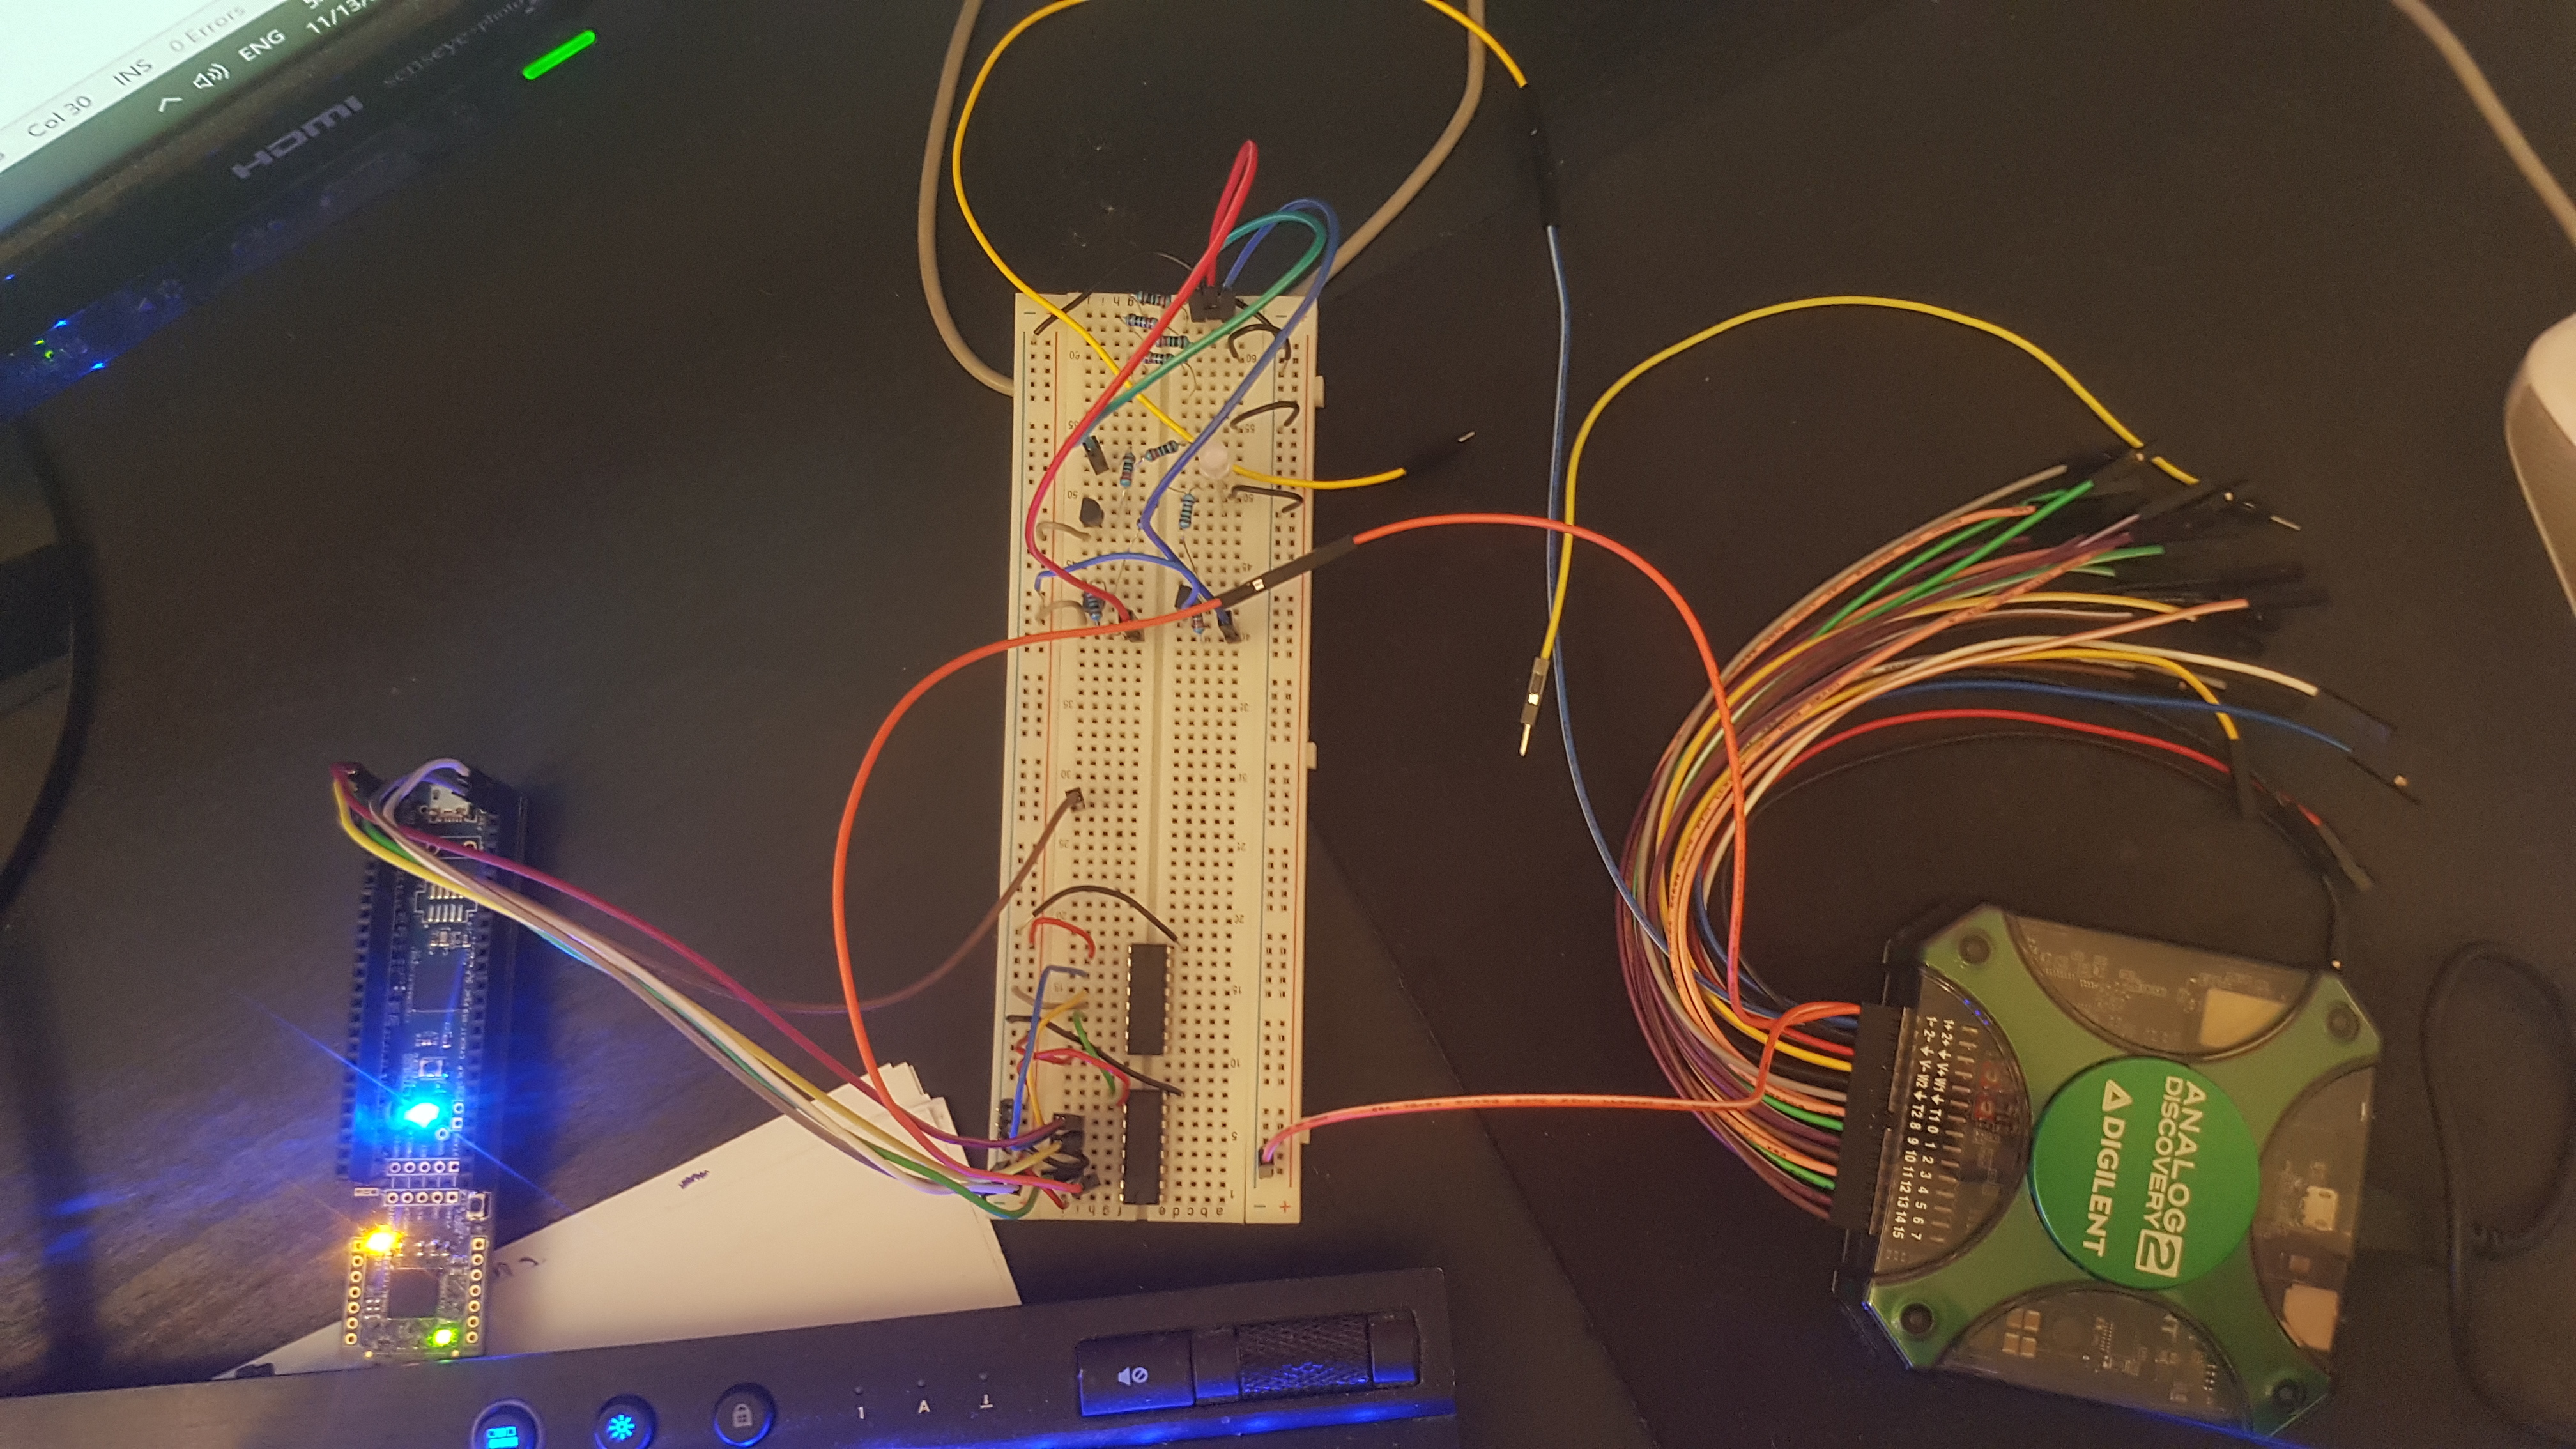
\includegraphics[width=\textwidth]{Modultest/CupLight/graphics/ShiftRegPWM_Test.jpg}
    \caption{Test opstilling for ShiftRegPWM opstilling}
    \label{fig:ShiftRegPWM_test}
\end{figure}

På opstillingen ses nederst i venstre hjørne PSoC'en, der har følgende ledninger forbundet til fumlebrættet i midten.

\begin{table}[H]
\centering
\begin{tabular}{|L{0.25\textwidth}|L{0.1\textwidth}|L{0.55\textwidth}|}
\hline
\textbf{Ledningsfarve} & \textbf{Navn} & \textbf{Funktion}                         \\ \hline
Lilla                  & sclk          & Clock der anvendes til shifting           \\ \hline
Gul                    & latch         & Pin der anvendes til at latche registeret \\ \hline
Grøn                   & mosi          & Pin hvor den serielle data shiftes til registeret \\ \hline
Hvid                   & Vdd           & Forsyning til fumlebræt                   \\ \hline
Grå                    & Gnd           & Ground til fumlebræt                      \\ \hline
\end{tabular}%

\end{table}

Til højre i figur \ref{fig:ShiftRegPWM_test} ses Analog Discovery2, der har en ledning til den første output pin af 74HC595 registeret.

\subsection{Test resultater og analyse for ShiftRegPWM}

Med denne opstilling og koden kompileret og skrevet ned på PSoC'en er det muligt at lave følgende målinger i WaveForms.
\\I figur \ref{fig:test_0_pin_0} ses den første test, der bare foretages ved en måling ved opstart.

\begin{figure}[H]
    \centering
    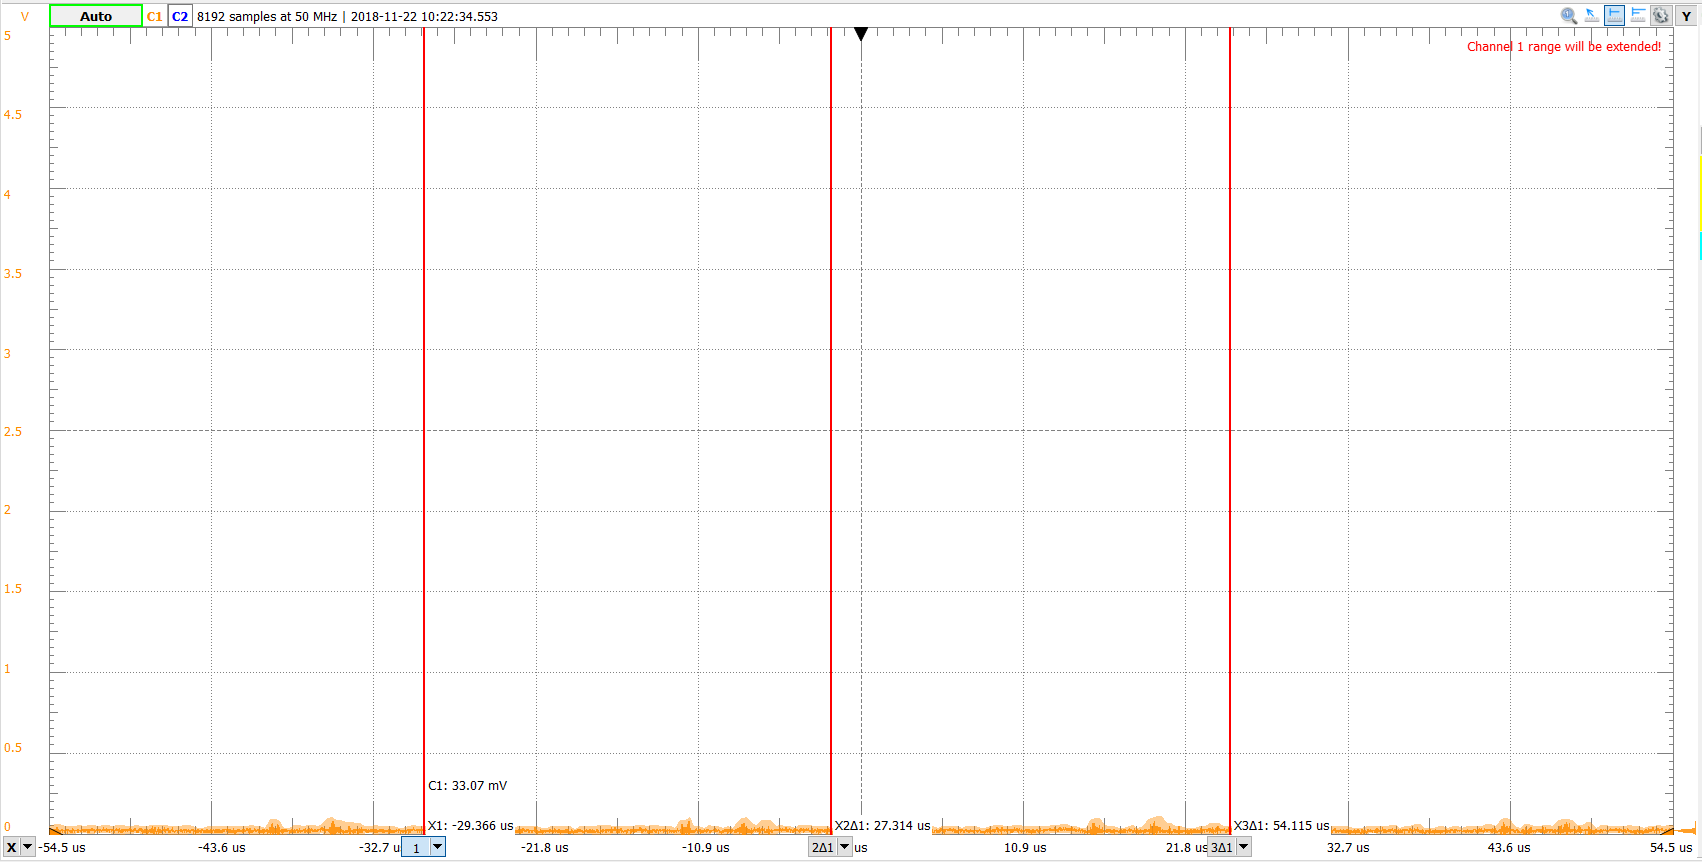
\includegraphics[width=\textwidth]{Modultest/CupLight/graphics/pwm_0.png}
    \caption{Test af setPin(0,0)}
    \label{fig:test_0_pin_0}
\end{figure}
Der kan ikke foretages meget analyse af denne andet, end det ses, at der ikke er noget PWM-signal herpå.

I figur \ref{fig:test_50_pin_0}, ses testen for at skrive værdien 50 til pin 0, ved brug af setPin-funktionen. 
\begin{figure}[H]
    \centering
    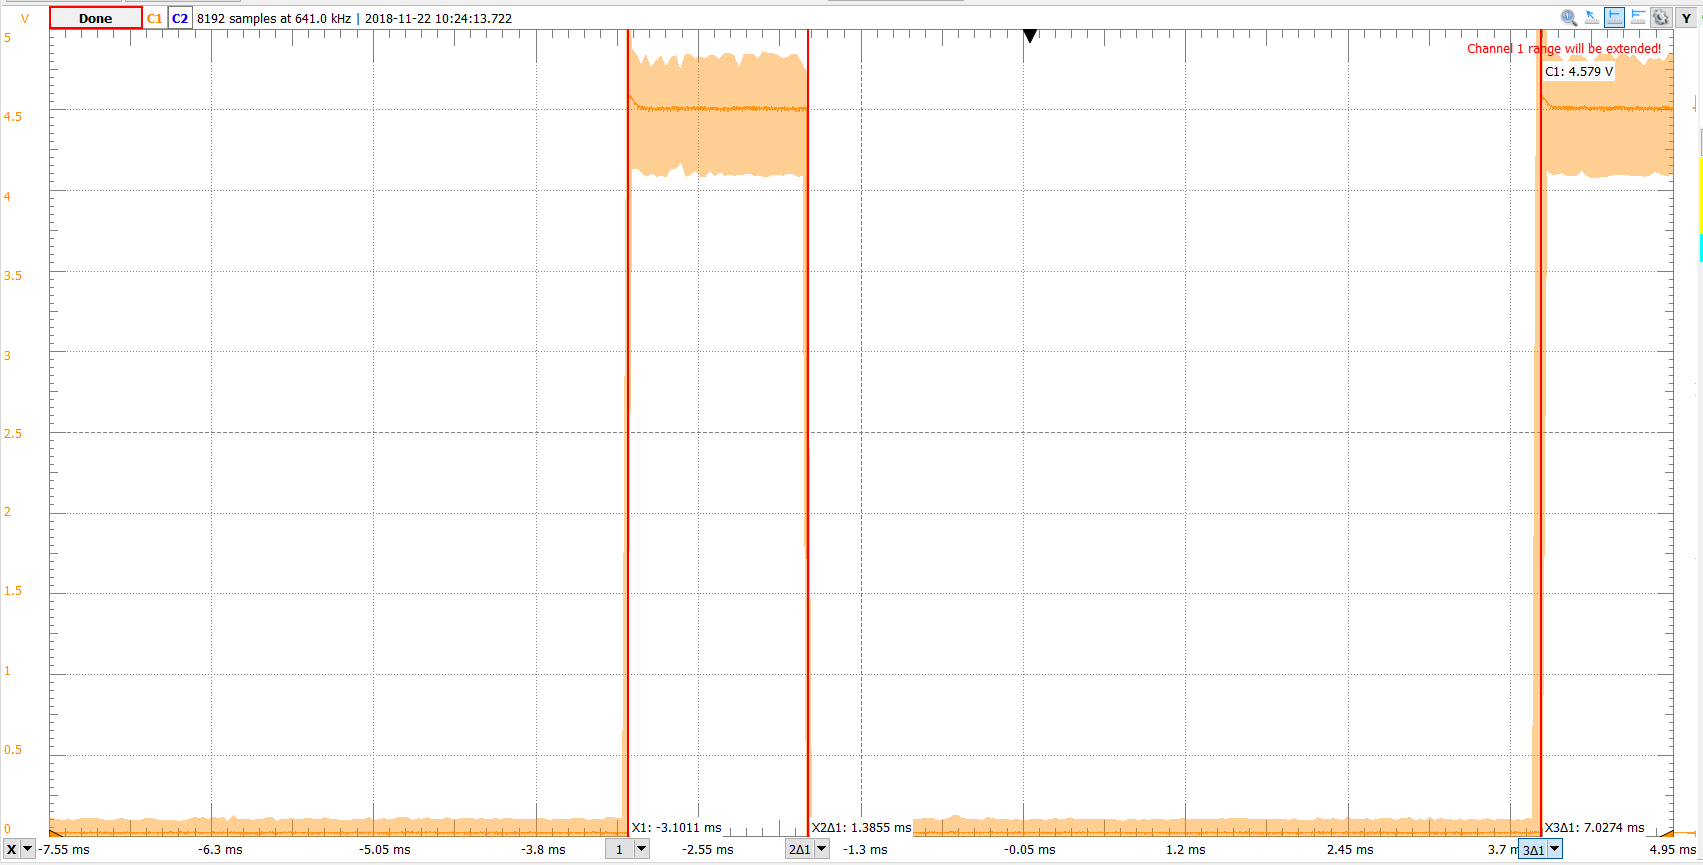
\includegraphics[width=\textwidth]{Modultest/CupLight/graphics/pwm_50.png}
    \caption{Test af setPin(0,50)}
    \label{fig:test_50_pin_0}
\end{figure}
Her aflæses det at PWM-signalet er tændt i 1.39ms ud af varigheden af en periode på  7.03 ms. Der kan altså her laves en beregning af den målte duty cycle ($dc_m$) og den forventede duty cycle ($dc_e$)
\begin{subequation}
\begin{align}
    \%dc_m=\frac{1.39ms}{7.03ms}\cdot 100\% = 19.8\%
    \\\%dc_e=\frac{50}{255}\cdot 100\% = 19.6\%
\end{align}
\end{subequation}
Det ses af ovenstående beregning at der er en forskel på +0.2\%  mellem den målte duty-cycle og den forventede duty-cycle.
\\Det andet man kan se af figuren er at frekvensen på PWM signalet er på $F_{pwm}=\frac{1}{7.03ms}=141Hz$. Denne frekvens er meget tilfredsstillende, da den blinker med en frekvens, der er høj nok til, at den ikke kan ses af mennesker. Det der er værd at medtage fra dette er, at frekvensen ikke kan bankes i vejret, da duty-cyclen på interrupt service rutinen vil blive større og derved vil, der ikke være time-slices nok for andre ting at køre. Derudover kan den heller ikke gøres meget mindre, da mennesker kan se frekvenser <60Hz. Dog er det værd at være opmærksom på, at der muligvis stadig kan hentes lidt her, hvis time-slices bliver et problem.

I figur \ref{fig:test_100_pin_0}, ses testen for at skrive værdien 100 til pin 0.
\begin{figure}[H]
    \centering
    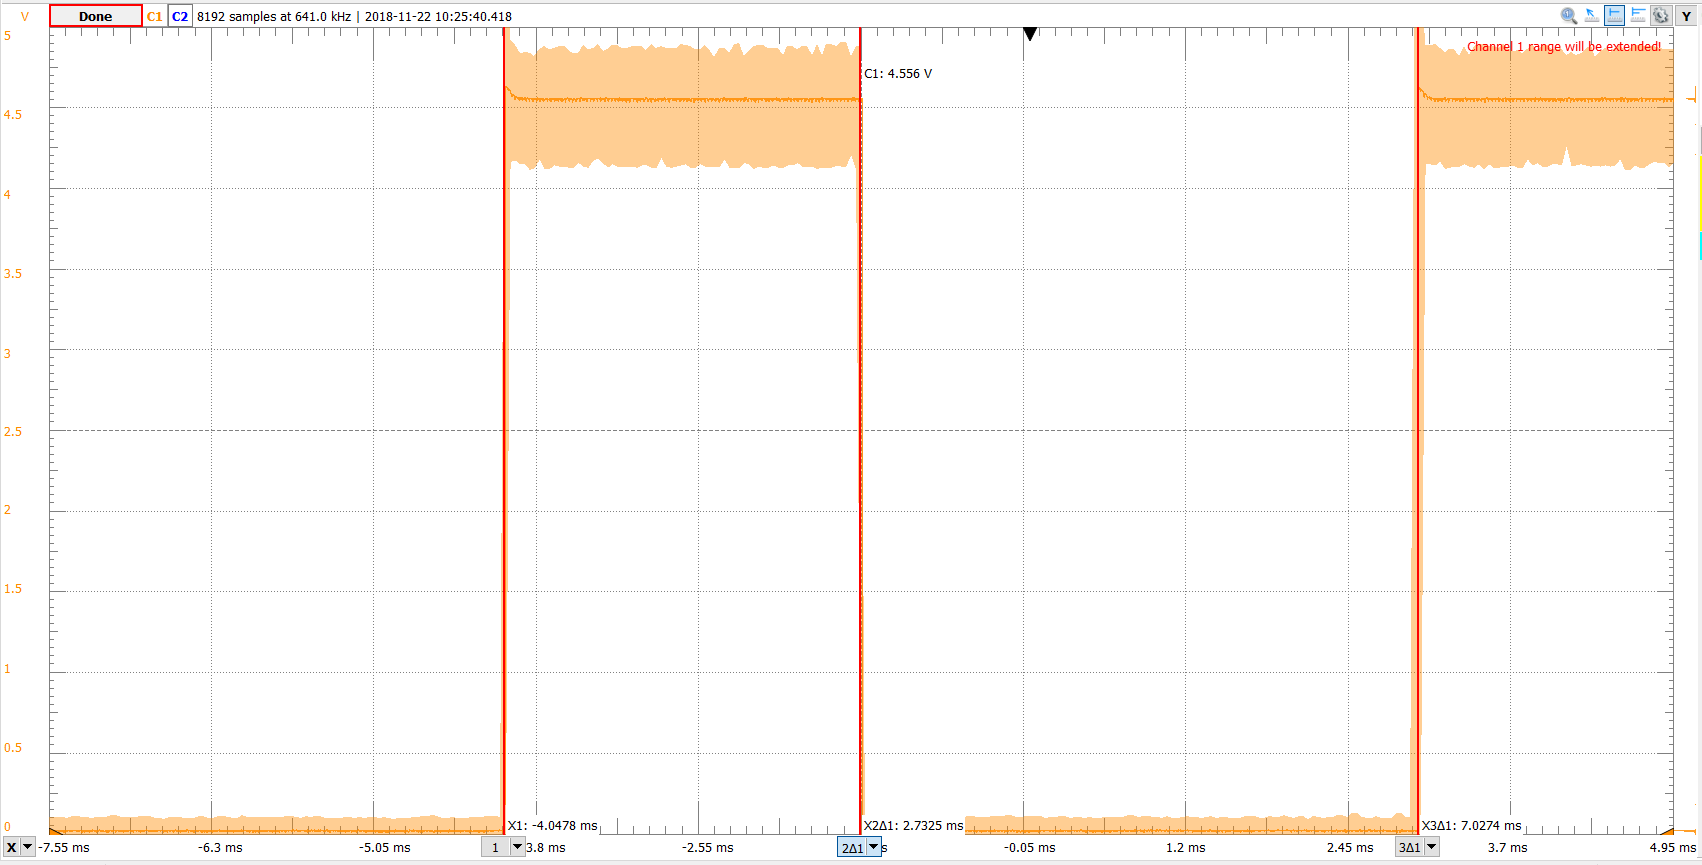
\includegraphics[width=\textwidth]{Modultest/CupLight/graphics/pwm_100.png}
    \caption{Test af setPin(0,100)}
    \label{fig:test_100_pin_0}
\end{figure}
Endnu en gang laves der en beregning mellem den målte og forventede duty-cycle,
\begin{subequation}
\begin{align}
    \%dc_m=\frac{2.73ms}{7.03}\cdot 100\% = 38.8\%
    \\\%dc_e=\frac{100}{255}\cdot 100\% = 39.2\%
\end{align}
\end{subequation}
Her ses det, at den forventede og målte er forskellige med -0.4\%, når der skrives værdien 100 til pin 0.

I figur \ref{fig:test_150_pin_0}, ses testen for at skrive værdien 150 til pin 0.
\begin{figure}[H]
    \centering
    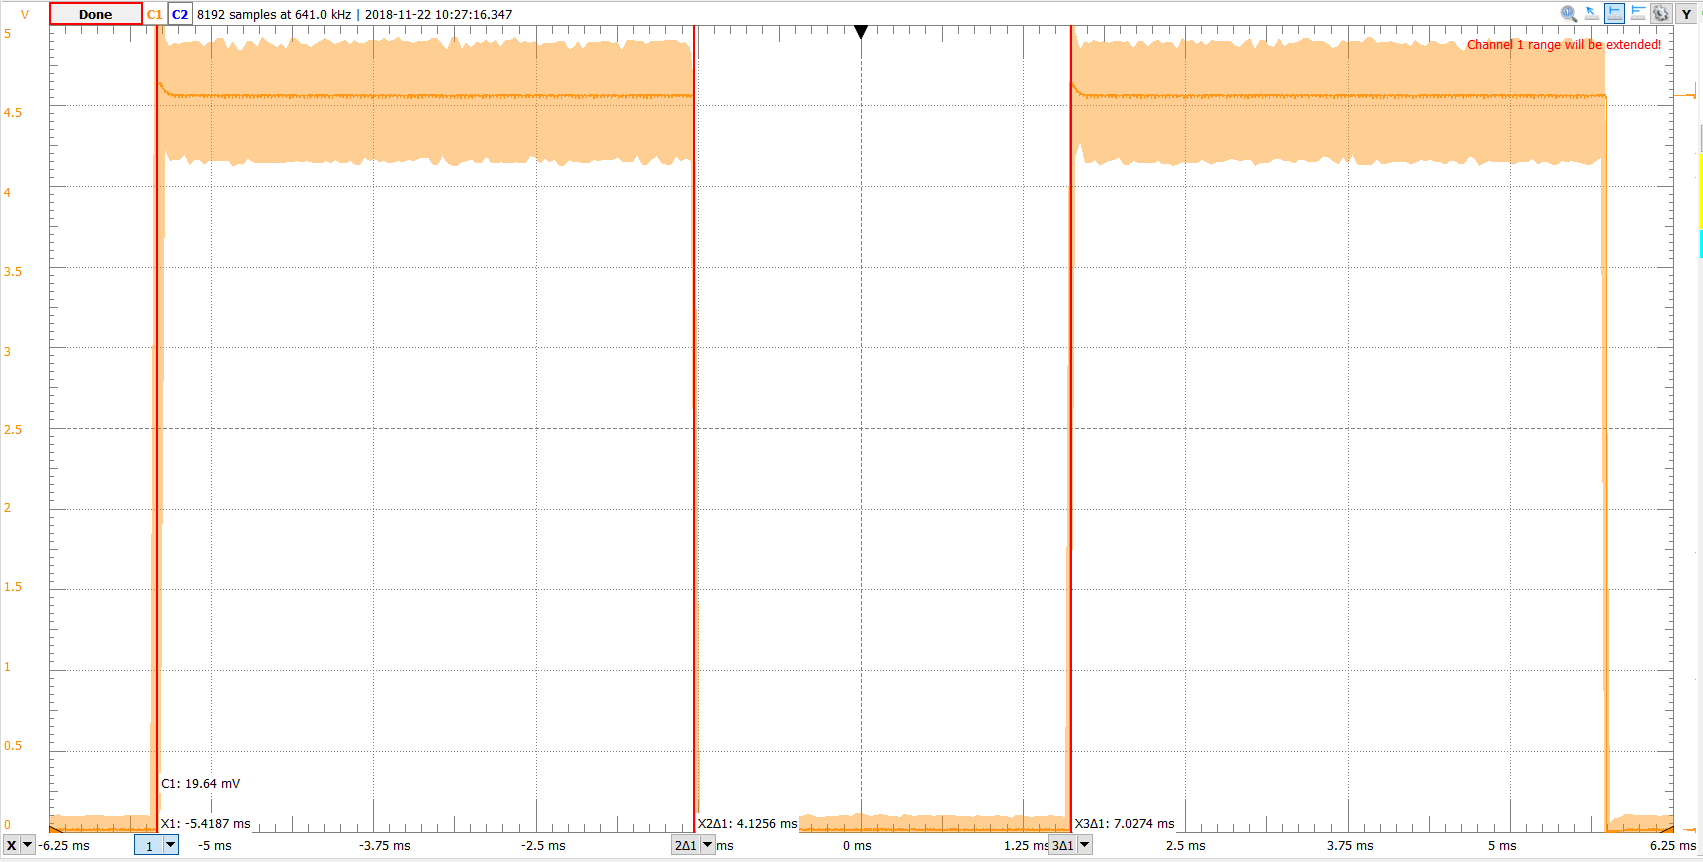
\includegraphics[width=\textwidth]{Modultest/CupLight/graphics/pwm_150.png}
    \caption{Test af setPin(0,150)}
    \label{fig:test_150_pin_0}
\end{figure}
Beregning af målt og forventet duty-cycle ses her.
\begin{subequation}
\begin{align}
    \%dc_m=\frac{4.13ms}{7.03ms}\cdot 100\% = 58.7\%
    \\\%dc_e=\frac{150}{255}\cdot 100\% = 58.8\%
\end{align}
\end{subequation}
Her ses at der er en forskel på +0.1\% mellem den målte og den forventede duty-cycle.

I figur \ref{fig:test_200_pin_0}, ses testen for at skrive værdien 200 til pin 0.
\begin{figure}[H]
    \centering
    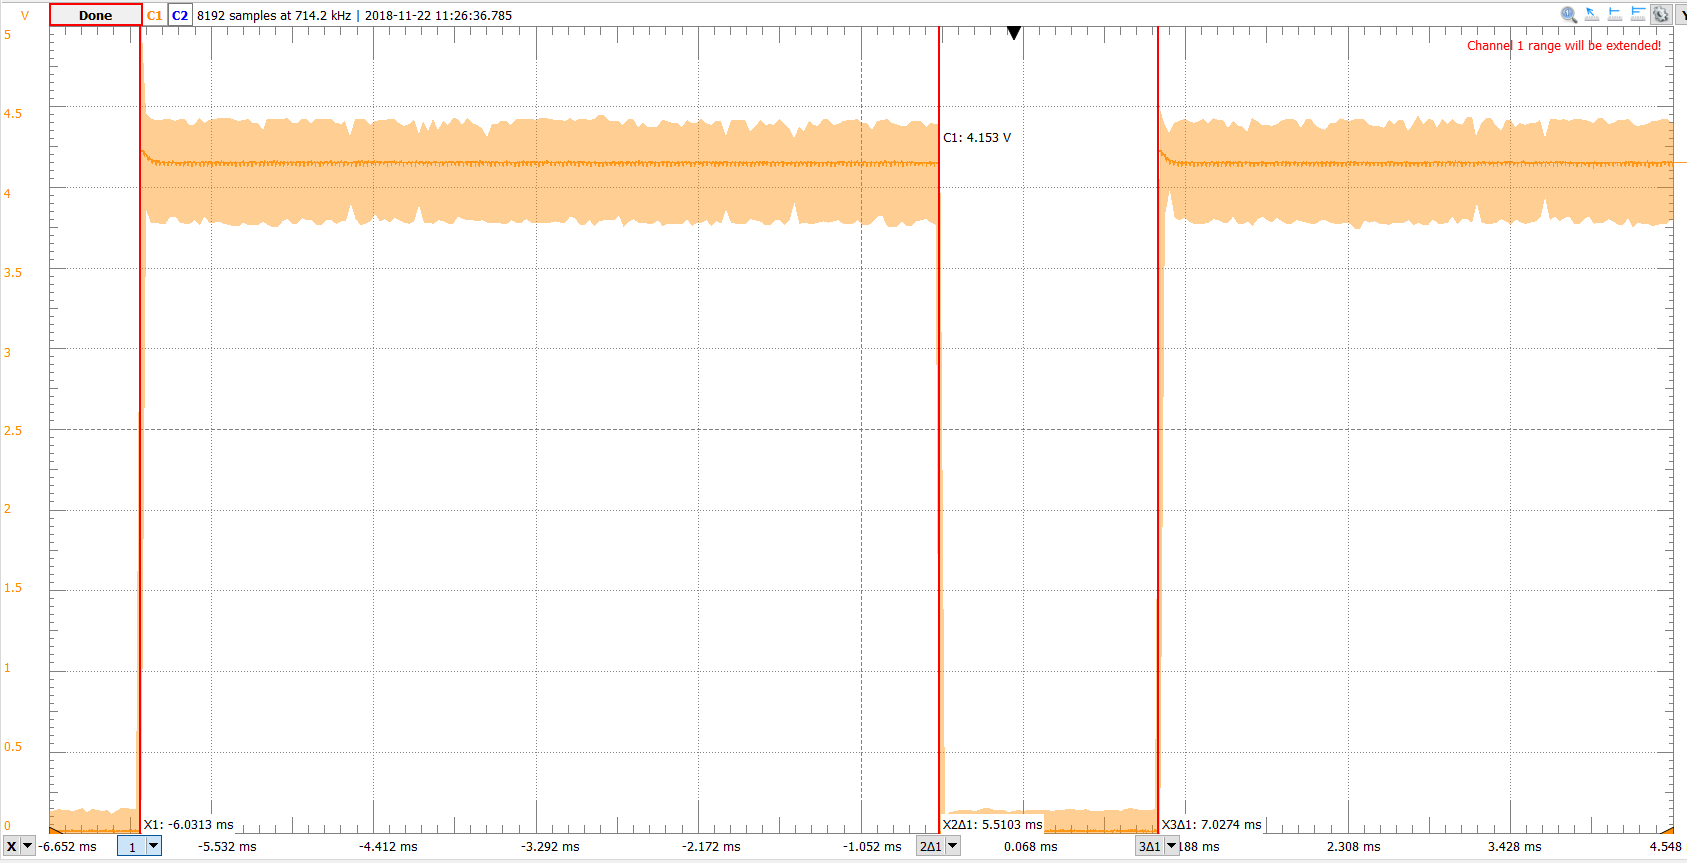
\includegraphics[width=\textwidth]{Modultest/CupLight/graphics/pwm_200.png}
    \caption{Test af setPin(0,200)}
    \label{fig:test_200_pin_0}
\end{figure}
Igen laves en beregning mellem målt og forventet duty-cycle.
\begin{subequation}
\begin{align}
    \%dc_m=\frac{5.51ms}{7.03}\cdot 100\% = 78.4\%
    \\\%dc_e=\frac{200}{255}\cdot 100\% = 78.4\%
\end{align}
\end{subequation}
Der findes, at der er en forskel på 0.0\% mellem den målte og forventede duty-cycle.

I figur \ref{fig:test_250_pin_0}, ses testen for at skrive værdien 250 til pin 0.
\begin{figure}[H]
    \centering
    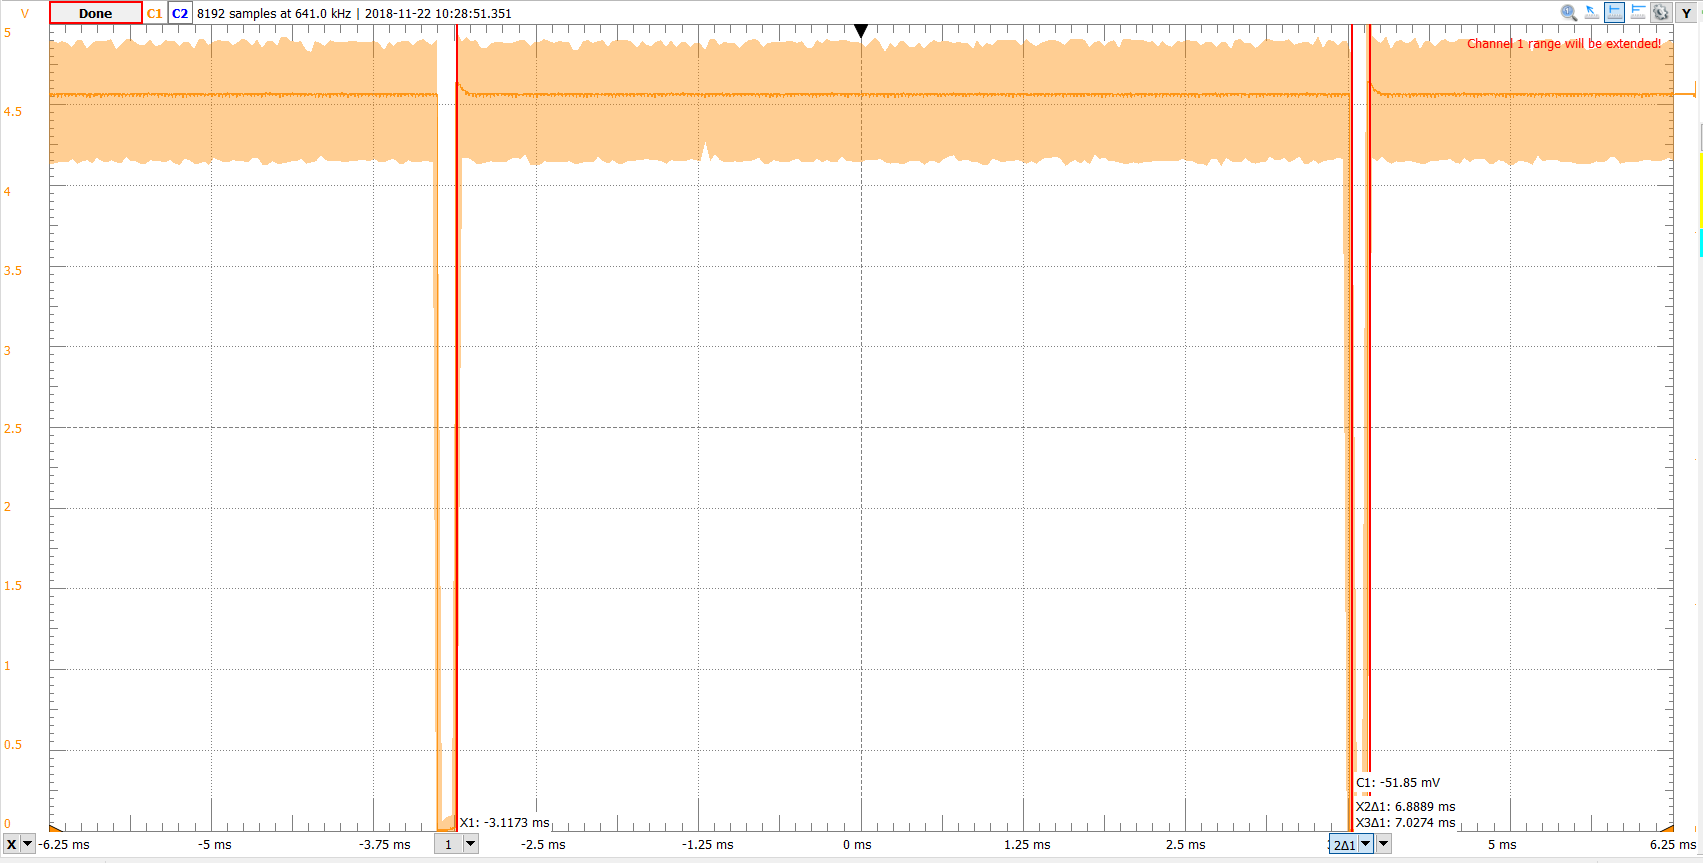
\includegraphics[width=\textwidth]{Modultest/CupLight/graphics/pwm_250.png}
    \caption{Test af setPin(0,250)}
    \label{fig:test_250_pin_0}
\end{figure}
\begin{subequation}
\begin{align}
    \%dc_m=\frac{6.89ms}{7.03}\cdot 100\% = 98.0\%
    \\\%dc_e=\frac{250}{255}\cdot 100\% = 98.0\%
\end{align}
\end{subequation}
Her ses at det, at den målte og forventede duty cycle er den samme.

I tabelen herunder ses alle målinger samlet, hvor den procentvise difference også er fundet.

\begin{table}[H]
\centering
\begin{tabular}{|l|l|l|}
\hline
\textbf{\%dc\_e} & \textbf{\%dc\_m} & \textbf{\%diff} \\ \hline
0                & 0                & 0               \\ \hline
19.6             & 19.8             & 1.01            \\ \hline
39.2             & 38.8             & 0               \\ \hline
58.8             & 58.7             & 1.02            \\ \hline
78.4             & 78.4             & 0               \\ \hline
98.0             & 98.0             & 0               \\ \hline
\end{tabular}%
\end{table}

Af tabellen kan man altså se at modulet i meget høj grad, virker som forventet i det værdierne der tilskrives registeret, rent faktisk danner et PWM-signal med den forventede duty-cycle, hvor der kun er en afvigelse på <2\%.\\
Den måling med størst afvigelse testes flere gange ved at genstarte PSoC, sætte PWM-signalet og måle det. Der blev lavet 10 målinger.



Der laves også en beregning af rise time for PWM-signalet.  Beregningen blev foretaget med et pwm-signal på 50\% dc.  Først laves der en måling på output pin af 74HC595, som det kan ses af figur \ref{cuplight_rise}.

\begin{figure}[H]
    \centering
    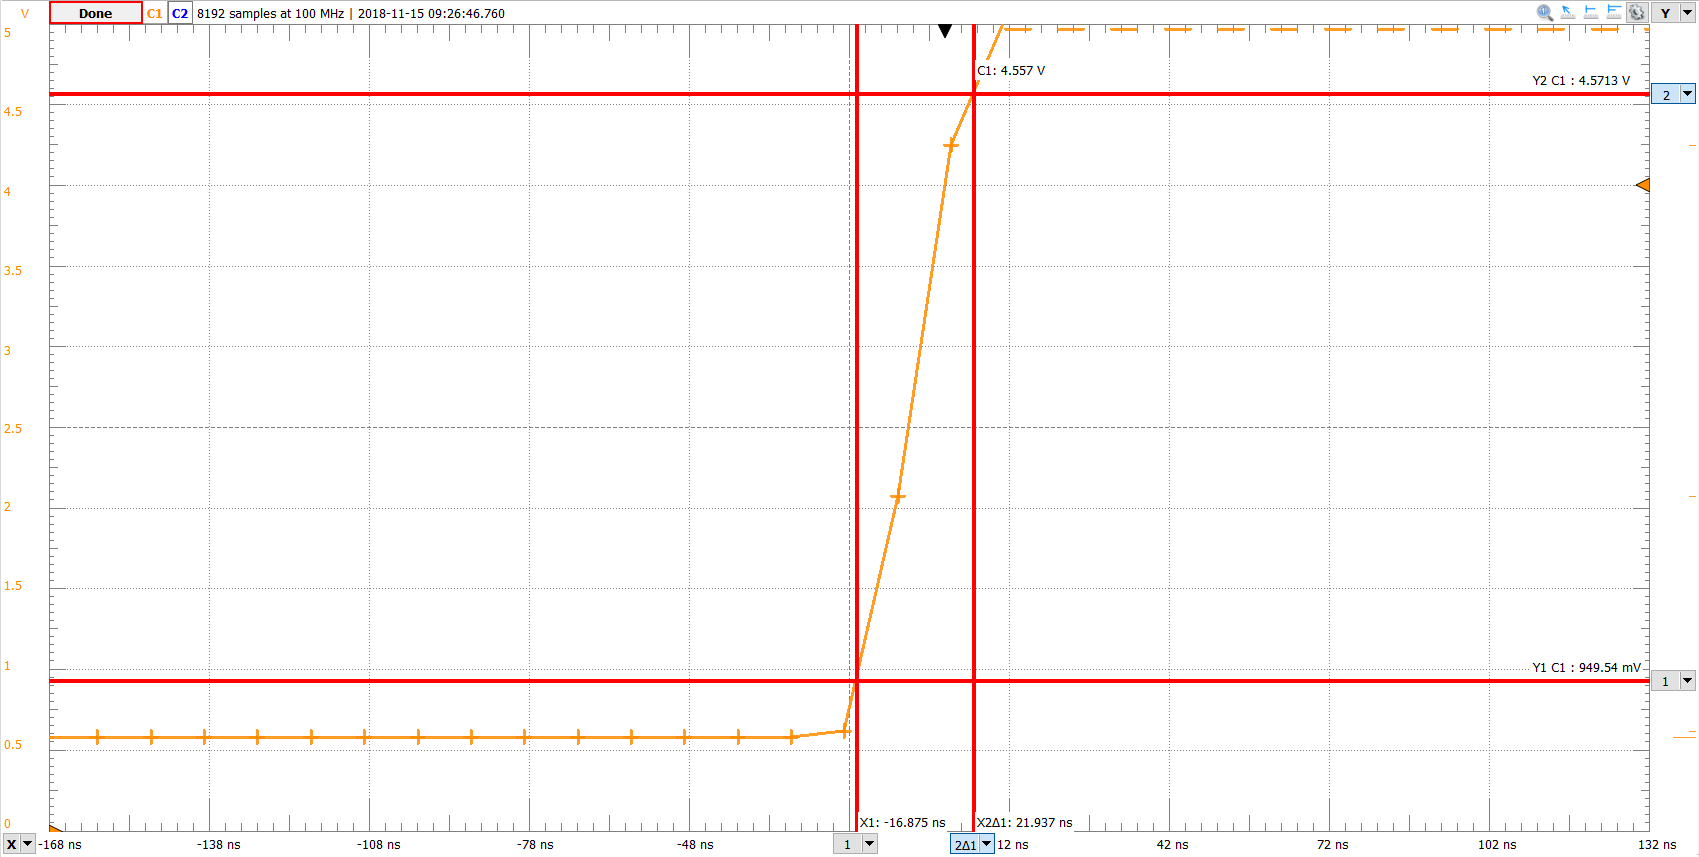
\includegraphics[width=\textwidth]{Modultest/CupLight/graphics/CupLight_rise_time.png}
    \caption{Den målte rise time ved 50\% dc}
    \label{fig:cuplight_rise}
\end{figure}

Af figur \ref{fig:cuplight_rise} ses det, at der på output pin af 74HC595 er et PWM-signal med en rise time på 21.9 ns. 
\\Herefter forbindes den testede pin til et transistor kredsløb som, det ses i hardware designet for den røde LED. Rise time kan nu testes i forhold til det, der når ud på LED'en. Denne måling kan ses i figur \ref{cuplight_rise_transistor}.

\begin{figure}[H]
    \centering
    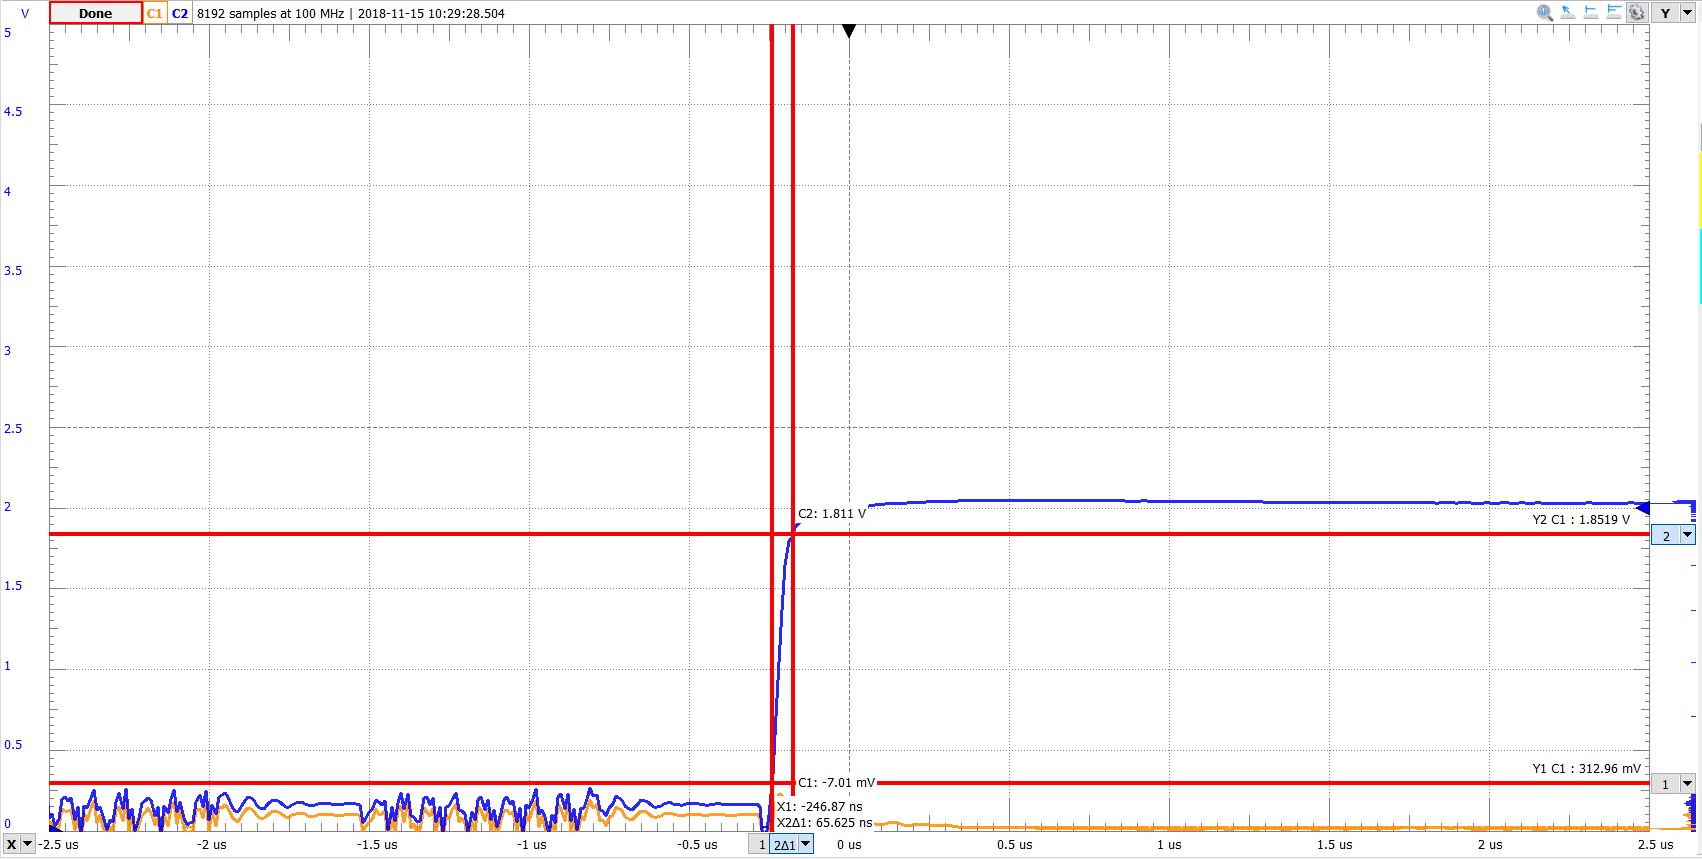
\includegraphics[width=\textwidth]{Modultest/CupLight/graphics/CupLight_rise_time_transistor.png}
    \caption{Den målte rise time ved 50\% dc over transistoren}
    \label{fig:cuplight_rise_transistor}
\end{figure}

På denne måling ses det først og fremmest at forward spænding af det, der ville være den rød led er 2.05V. Derudover ses det også at rise time på LED'en er 65.6 ns.

Da controlleren for PSoC skal kunne håndtere flere interrupts service rutine, er det også relevant at teste varigheden af interrupt service rutinen til opdatering. Det er især relevant fordi interrupt service rutinen for lyset er rimelig heavy duty, da den kaldes mange gange i sekundet. Måden det blev testet på var at sætte en pin høj, ved indgangen til interrupt rutinen og sætte den lav igen ved udgangen af interrupt rutinen. Koden for dette ses i listing \ref{lst:isr_length_code}
\begin{lstlisting}[caption={Kode for at teste længden af interrupt service rutinen}, label={lst:isr_length_code}]
CY_ISR(updater_handler)
{
    Pin_update_time_Write(1);
    update(); //The update routine
    Pin_update_time_Write(0);
}  
\end{lstlisting}

Køres koden i listing  \ref{lst:isr_length_code} fås følgende figur \ref{fig:cuplight_isr_length}.

\begin{figure}[H]
    \centering
    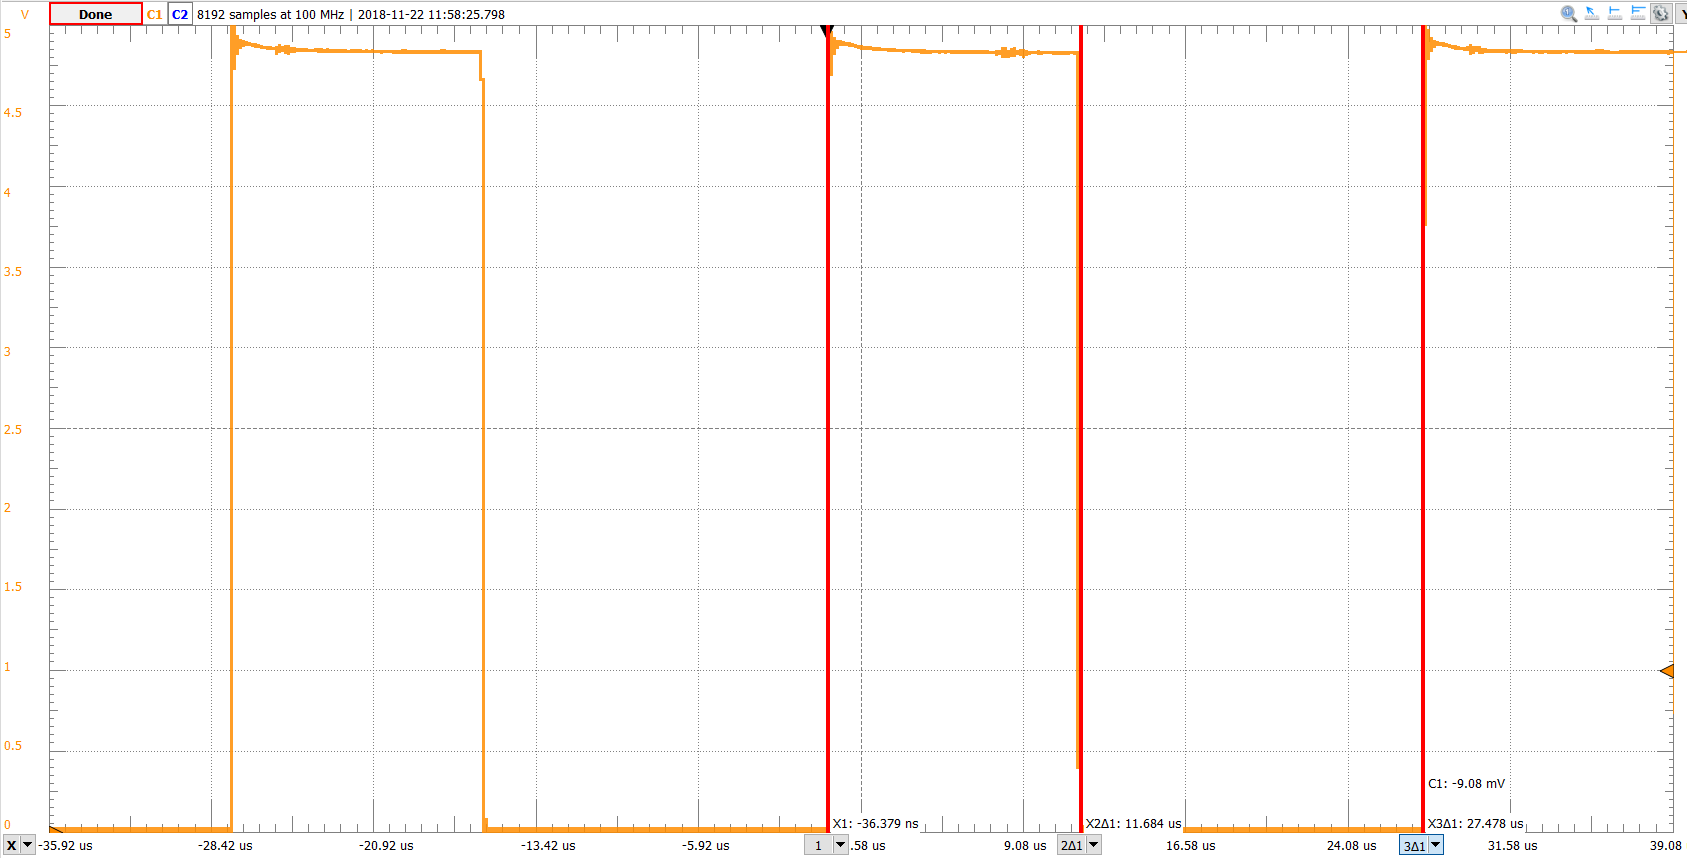
\includegraphics[width=\textwidth]{Modultest/CupLight/graphics/Test_isr_length.png}
    \caption{Test af længden på ISR til opdatering af cup}
    \label{fig:cuplight_isr_length}
\end{figure}

Af figur \ref{fig:cuplight_isr_length} ses det, at der som forventet at interrupt service rutinene kaldes mange gange i sekundet. Af figuren ses det at der perioden eller tiden mellem hvert interrupt er 27.3us. Dette vil sige at der interruptes med en frekvens på $F=\frac{1}{27.3us}=36630Hz$. Af denne periode, varer interrupt rutinen $t=11.7us$. Det giver altså en duty cycle på $\%dc=\frac{11.7us}{27.3us}\cdot 100\%=43\%$. Det kan altså sige, at selvom denne interrupt service rutine, måske ikke varer særlig lang tid, så tager den stadig en stor del af time-slices. 

\subsection{CupLight\_IF modul test}
Efter af have testet, at ShiftRegPWM modulet leverede et tilfredsstillende PWM-signal, så er det nu muligt at teste og anvende interfacet CupLight\_IF til at styre lys. Af kravspecifikationen under ikke-funktionelle krav \fullref{kravspec:sec:ikke_funktionelle_krav} ses det, at lyset skal kunne lyse med 10 forskellige farver. Dette skal selvfølgelig testes heri.
\subsection{Test opstilling for ShiftRegPWM}
Til at teste CupLight\_IF blev, der igen anvendt et testprogram, der principielt minder ufatteligt meget om det forrige. Det anvendte testprogram kan ses i listing \ref{lst:CupLight_Test}.

\begin{lstlisting}[caption={Test program for CupLight_IF}, label={lst:CupLight_Test}]

#include <stdbool.h>
#include "project.h"
#include "ShiftRegPWM.h"
#include "CupLight_IF.h"

#define LEDTOTEST 2

CY_ISR_PROTO(ISR_UART_rx_handler);
void handleByteReceived(uint8_t byteReceived);

uint8_t globalRed = 0;
uint8_t globalGreen = 0;
uint8_t globalBlue = 0;

int main(void)
{
    CyGlobalIntEnable; /* Enable global interrupts. */
    isr_uart_rx_StartEx(ISR_UART_rx_handler);
    UART_1_Start();
    UART_1_PutString("Program started\r\n"); 
    initShiftRegPWM();
    for(;;)
    {
    }
}

CY_ISR(ISR_UART_rx_handler)
{
    uint8_t bytesToRead = UART_1_GetRxBufferSize();    
    //Read bytes
    while (bytesToRead > 0)
    {
        uint8_t byteReceived = UART_1_ReadRxData();
        UART_1_WriteTxData(byteReceived); // echo back
        
        handleByteReceived(byteReceived);
        
        bytesToRead--;
    }
}

void handleByteReceived(uint8_t byteReceived)
{
    switch(byteReceived)
    {
        case 'q' :
        {
            globalRed = 255;
            controlLight(LEDTOTEST,(color_t){globalRed,globalGreen,globalBlue});
        }
        break;
        case 'w' :
        {
            globalGreen = 255;
            controlLight(LEDTOTEST,(color_t){globalRed,globalGreen,globalBlue});
        }
        break;
        case 'e' :
        {
            globalBlue = 255;
            controlLight(LEDTOTEST,(color_t){globalRed,globalGreen,globalBlue});
        }
        break;
        case 'a' :
        {
            globalRed += 5;
            controlLight(LEDTOTEST,(color_t){globalRed,globalGreen,globalBlue});
        }
        break;
        case 's' :
        {
            globalGreen += 5;
            controlLight(LEDTOTEST,(color_t){globalRed,globalGreen,globalBlue});
        }
        break;
        case 'd' :
        {
            globalBlue += 5;
            controlLight(LEDTOTEST,(color_t){globalRed,globalGreen,globalBlue});
        }
        break;
        break;
        default :
        {
            // nothing
        }
        break;
    }
}
\end{lstlisting}

Den største forskel i dette forskel er anvendelsen af typen $color_t$ til at styre farven, og i stedet for at sætte en pin, så sættes et helt lys (RGB-led). Der anvendes også 3 globale variable, der bruges til stepvis at styre lyset.

Den fysiske opstilling til testen, er en forsimplet version af den skematiske fra Hardware designet for CupLight. Det vil altså sige, at der kun styres en LED til en start. Selvfølgelig er det ikke optimalt, at der kun styres en LED, når der er 5 i en kopholder, men der blev brugt de ressourcer, der var til rådighed. Opstillingen ses i figur \ref{fig:cupLight_test}

\begin{figure}[H]
    \centering
    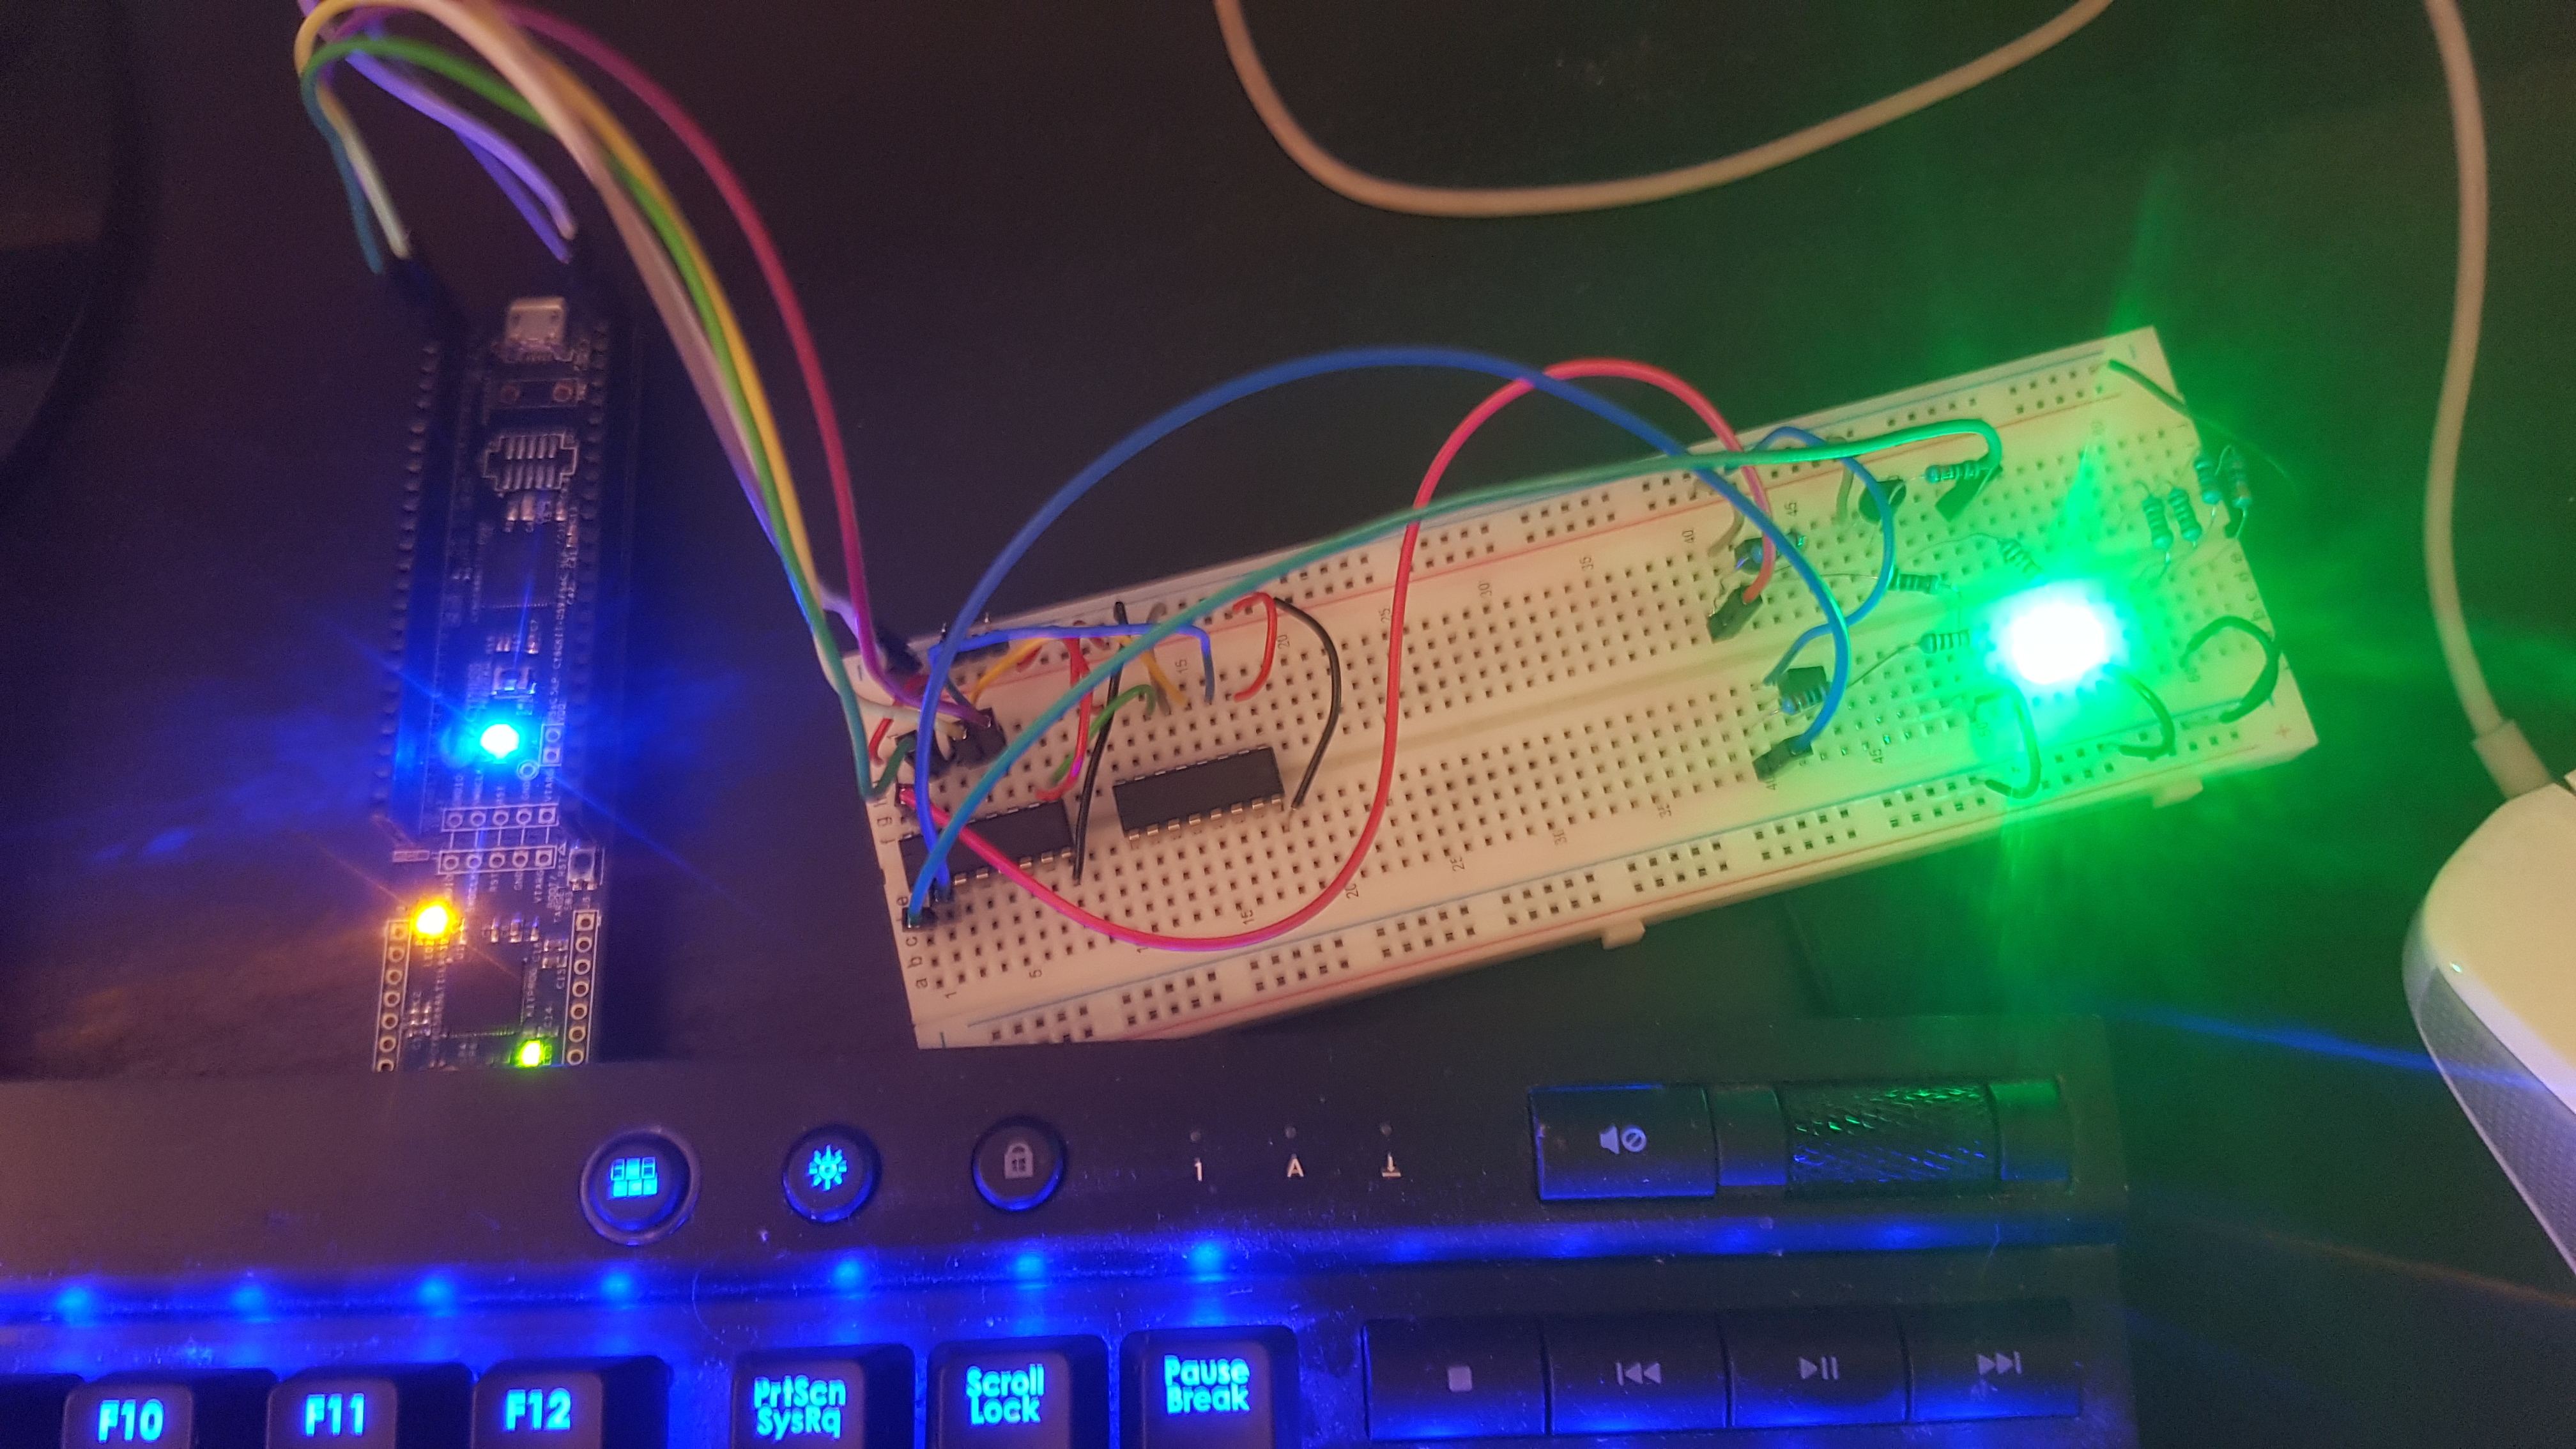
\includegraphics[width=\textwidth]{Modultest/CupLight/graphics/CupLight_IF_TEST.jpg}
    \caption{Test opstilling for CupLight\_IF og CupLight Hardware}
    \label{fig:cupLight_test}
\end{figure}

Interfacet blev herved testet, om det kunne styre farven af en LED ved at skrive den ønskede farve til LED'en med det ønskede nummer. Da der skal anvendes 3 pins pr. LED blev der først testet med LED'en forbundet til de tre første pins [0;2] og herefter[3;5]. Da der der ikke er nok pins tilbage på et shiftRegister, blev der daisy-chained et mere og pins[6:7] på det første shiftregister og pin[0] på det andet shiftregister blev tilsluttet LED'en som en tredje test. For at vise at hvert led kan lyse med hver sin farve så tændes LED'erne 0,1 og 2 med henholdsvis farverne Rød,Grøn og Blå. Resultatet af disse test kan ses i de efterfølgende figurer. Her er det vigtigt, at se hvordan forbindelserne mellem 74HC595 og LED'erne skifter.

\begin{figure}[H]
    \centering
    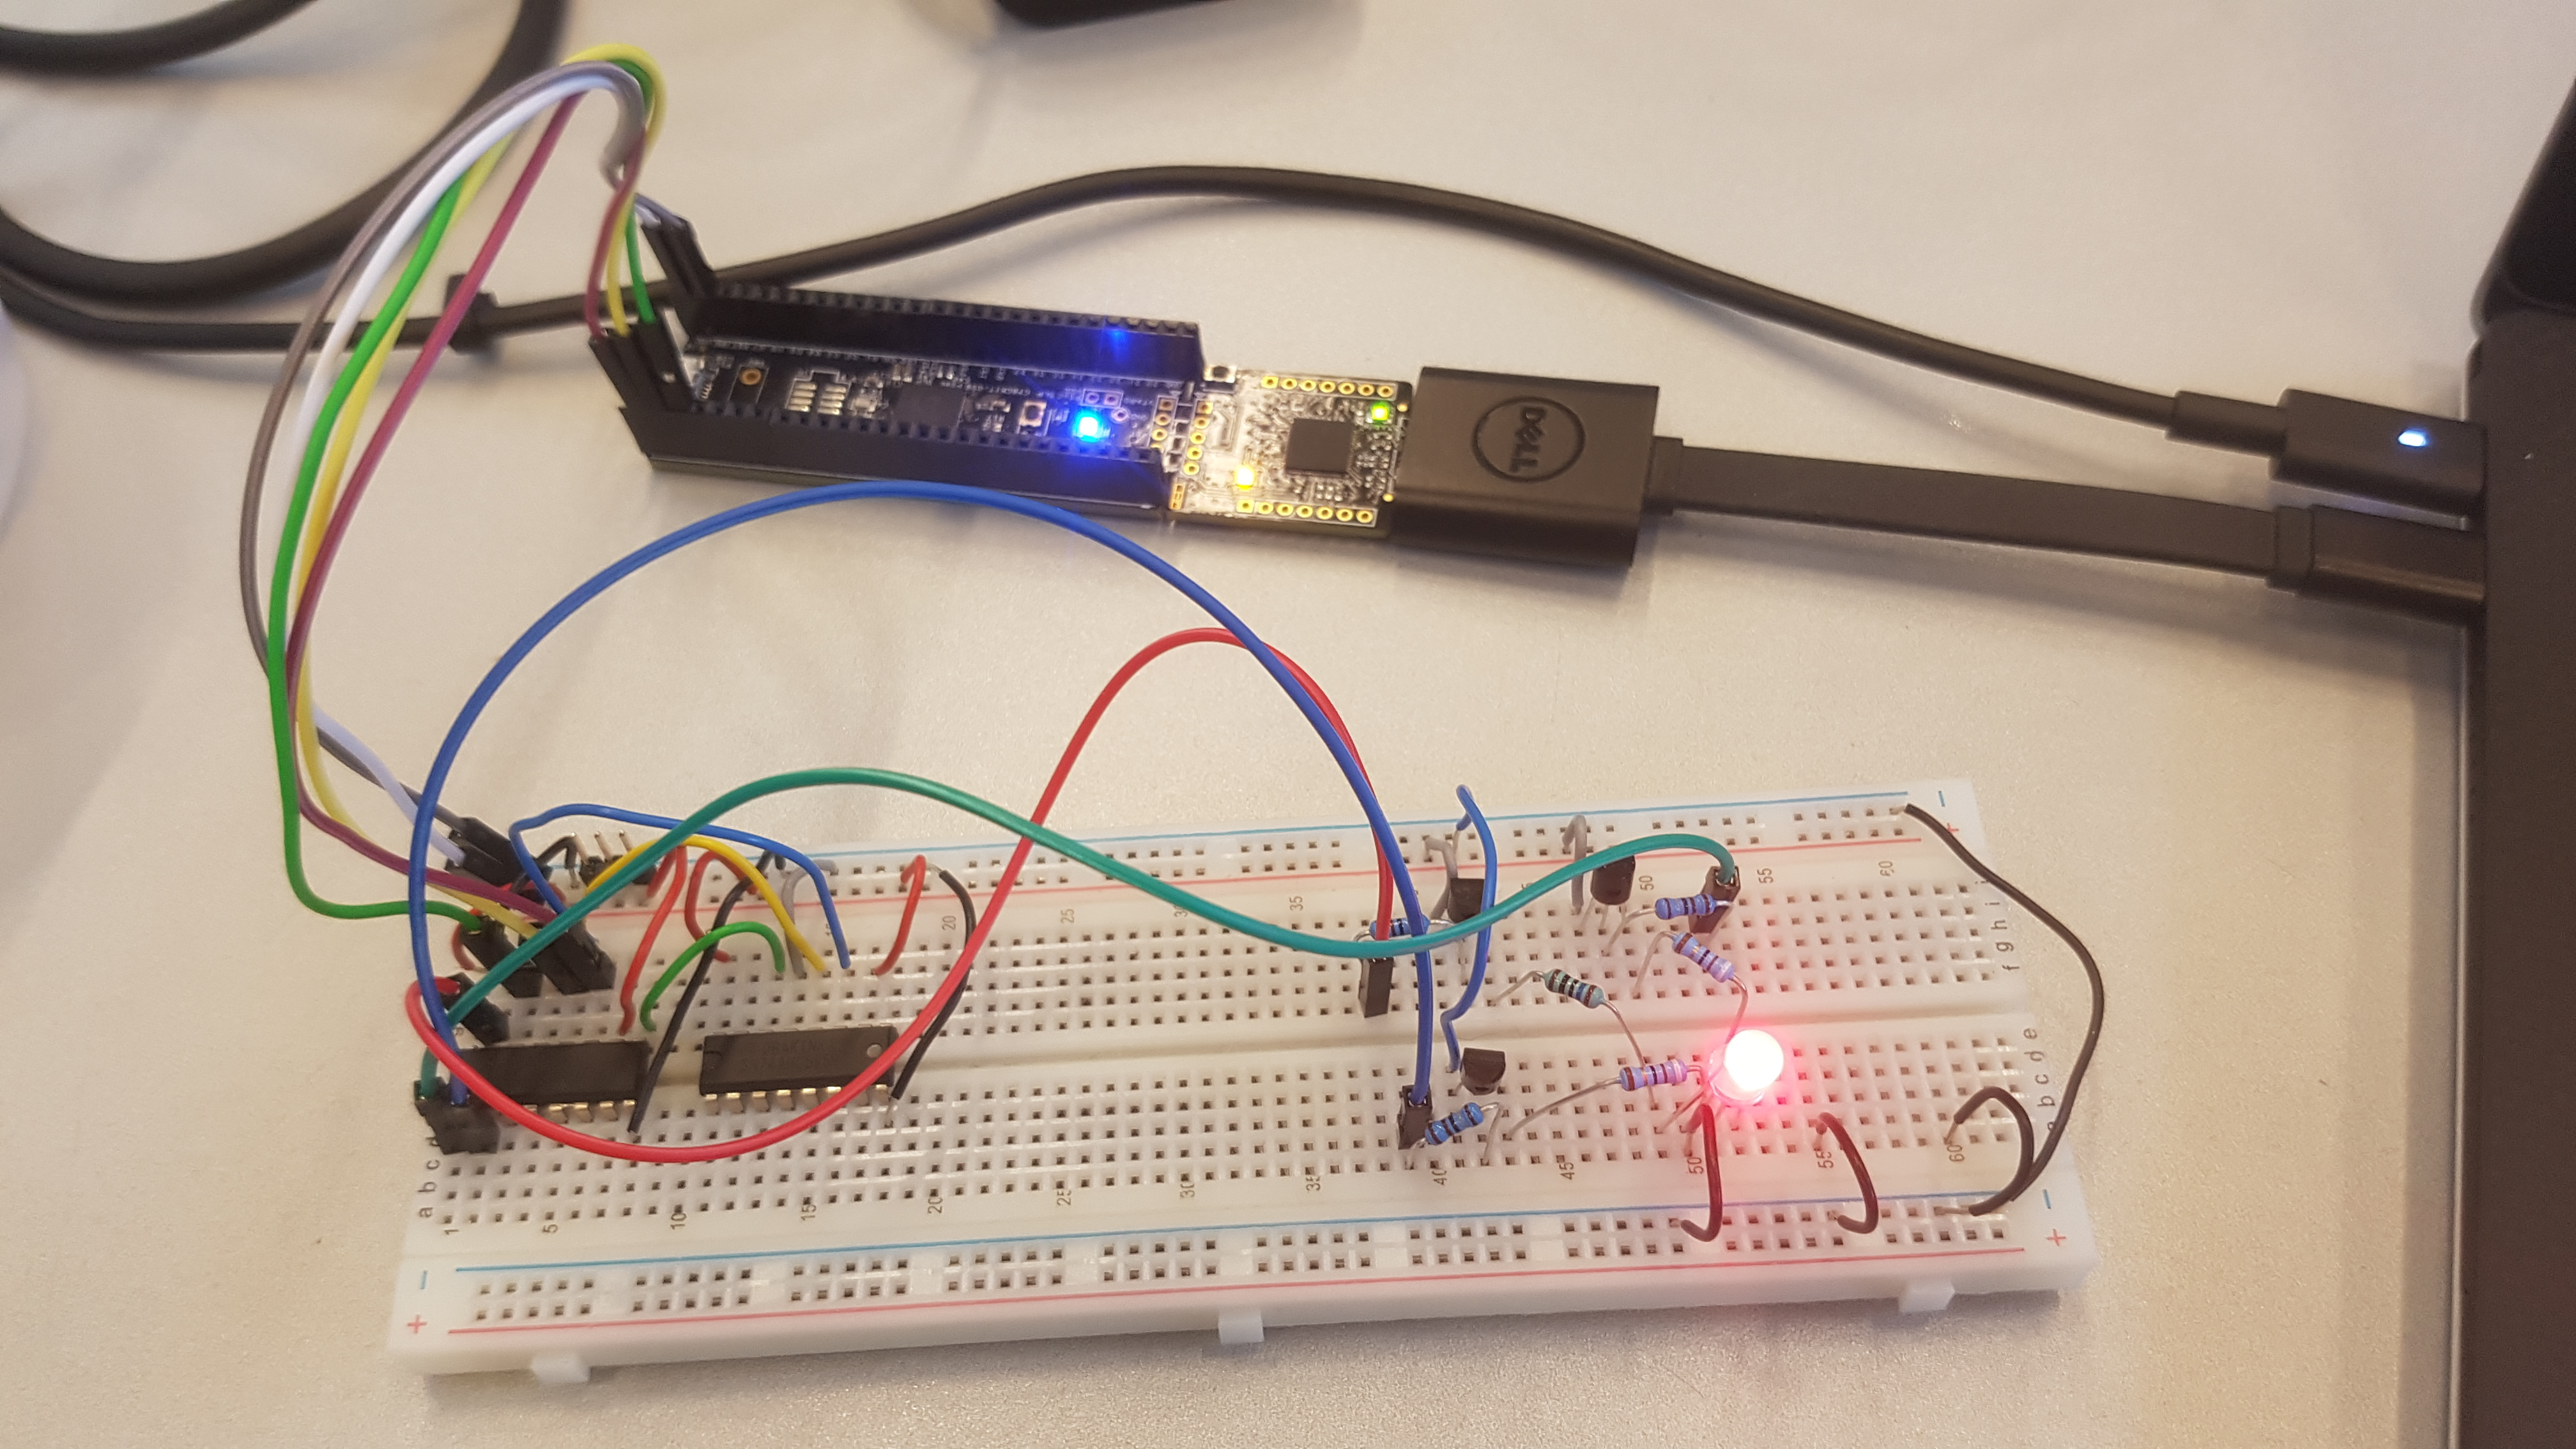
\includegraphics[width=\textwidth]{Modultest/CupLight/graphics/interface_test1.jpg}
    \caption{Test af controlLight(0,RED)}
    \label{fig:cuplight_red_test1}
\end{figure}

\begin{figure}[H]
    \centering
    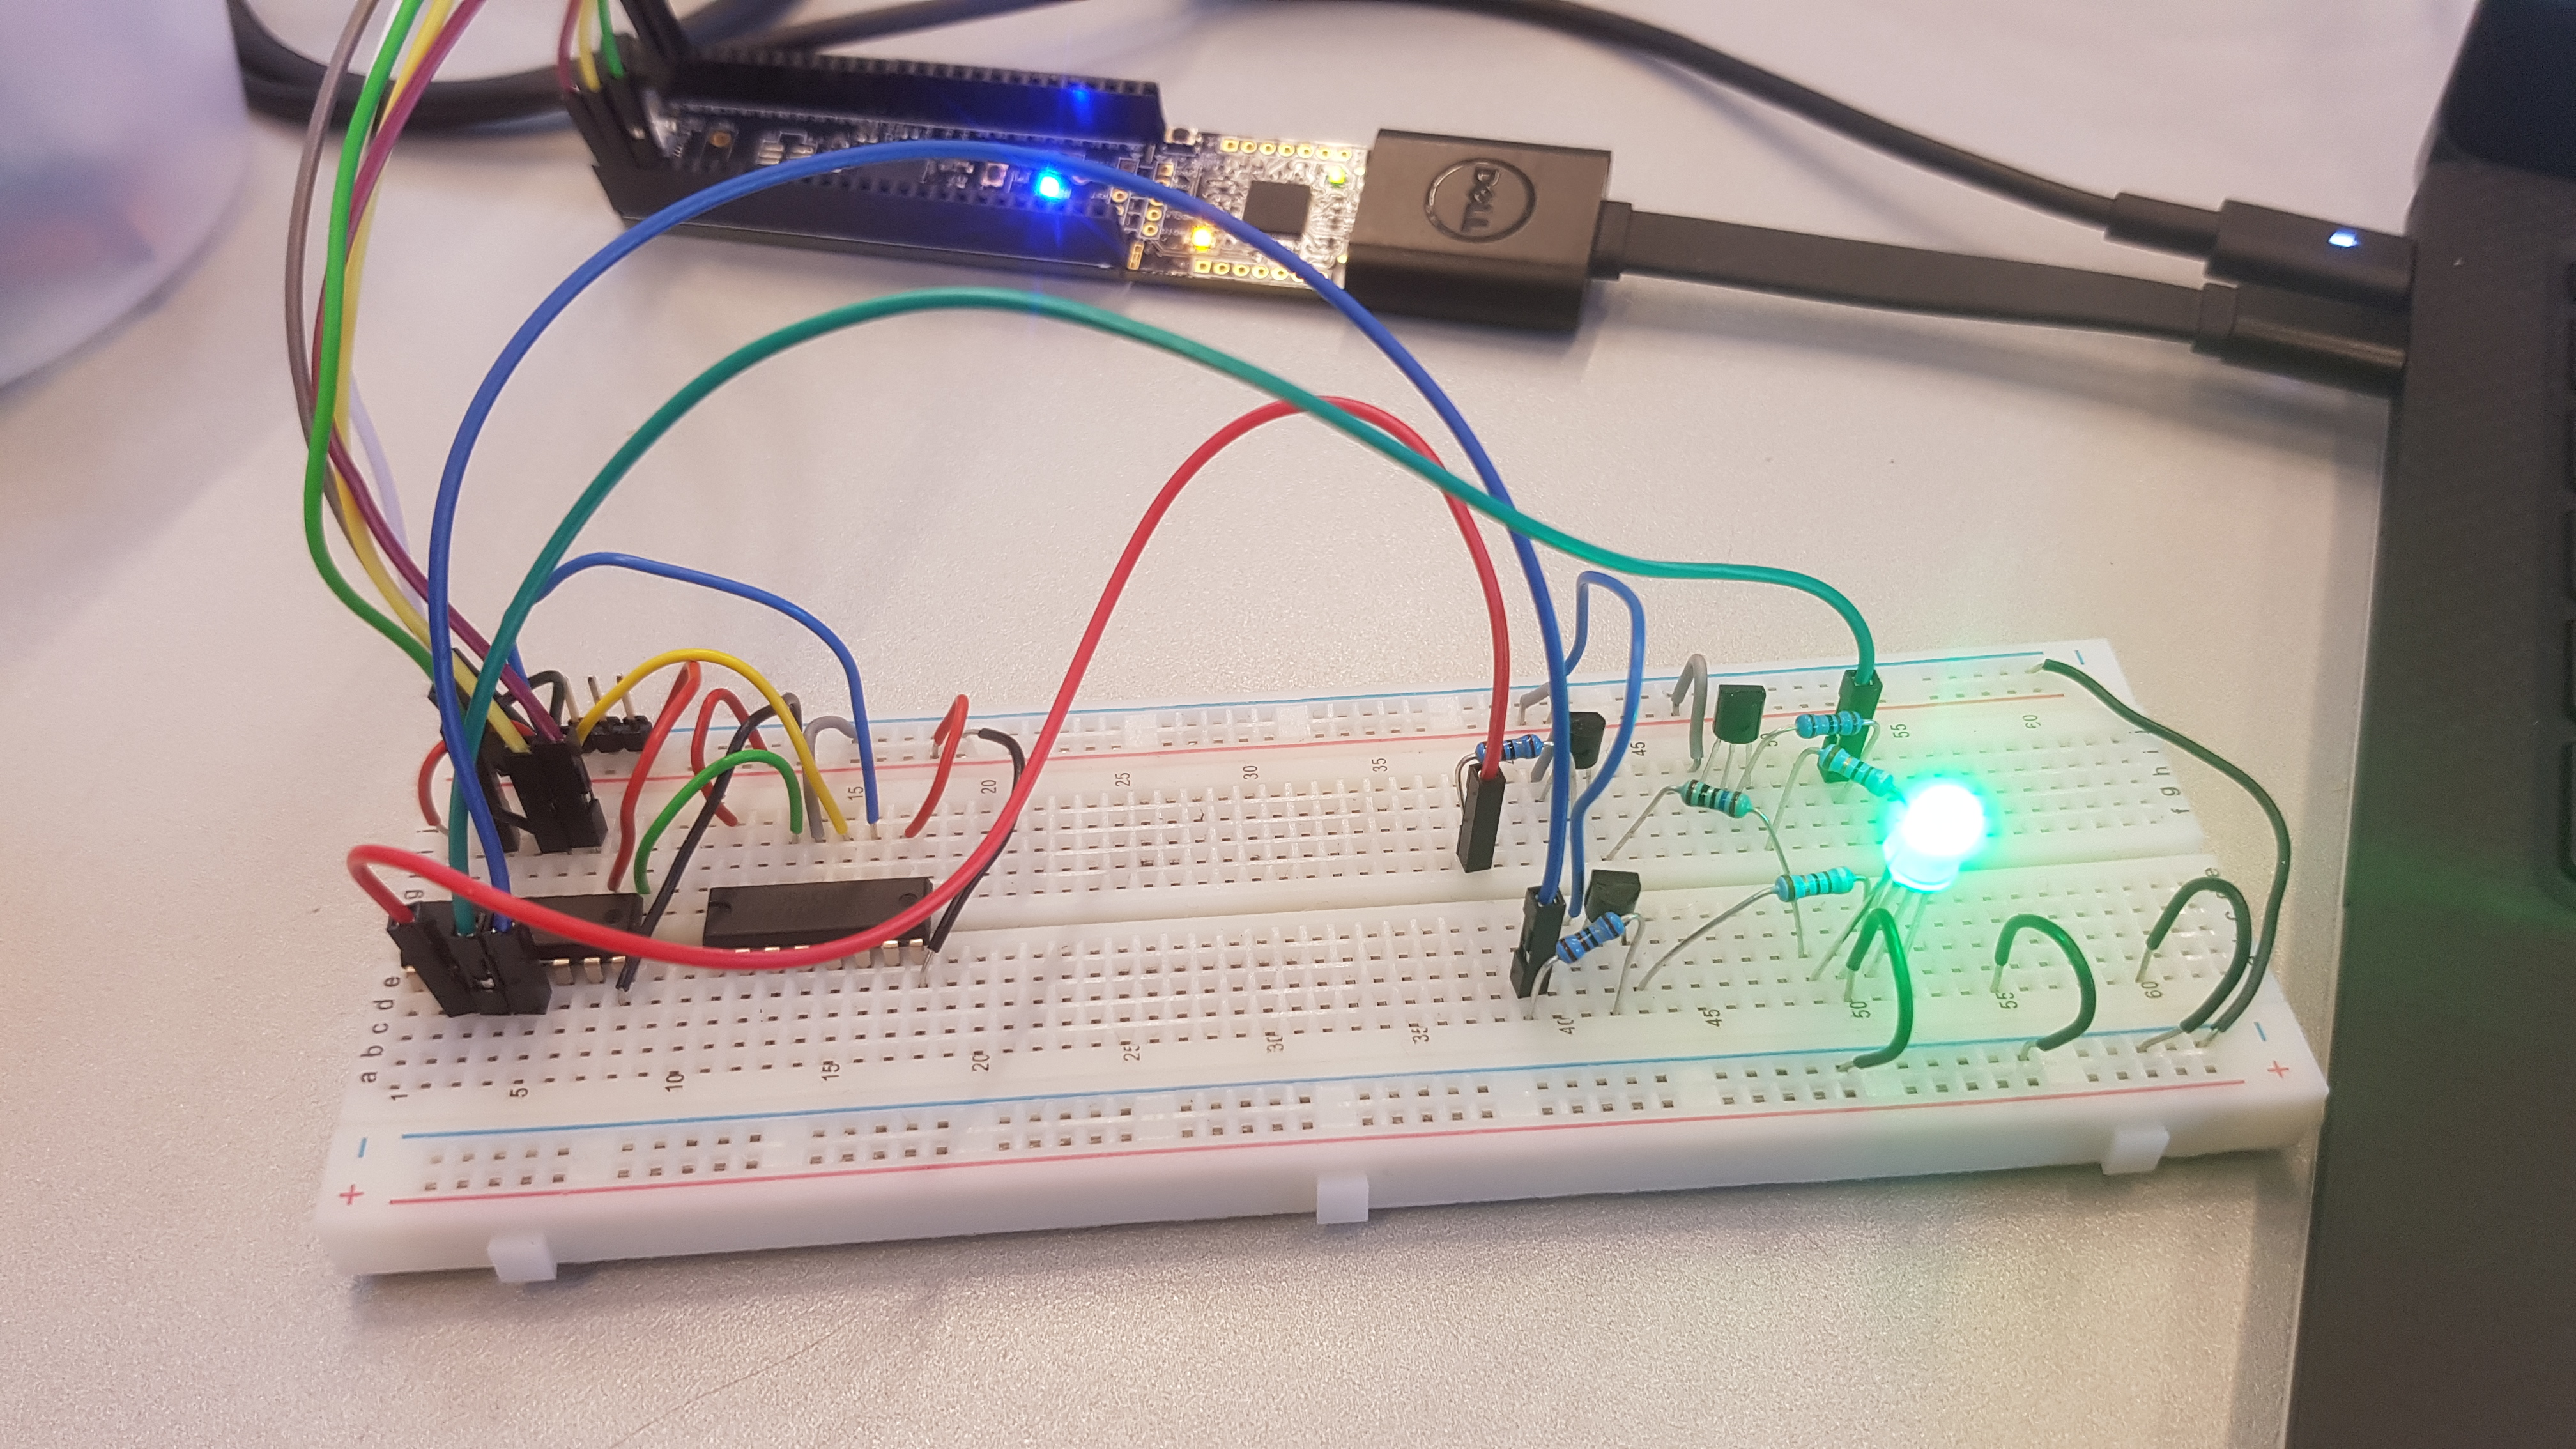
\includegraphics[width=\textwidth]{Modultest/CupLight/graphics/interface_test2.jpg}
    \caption{Test af controlLight(1,GREEN)}
    \label{fig:cuplight_green_test2}
\end{figure}

\begin{figure}[H]
    \centering
    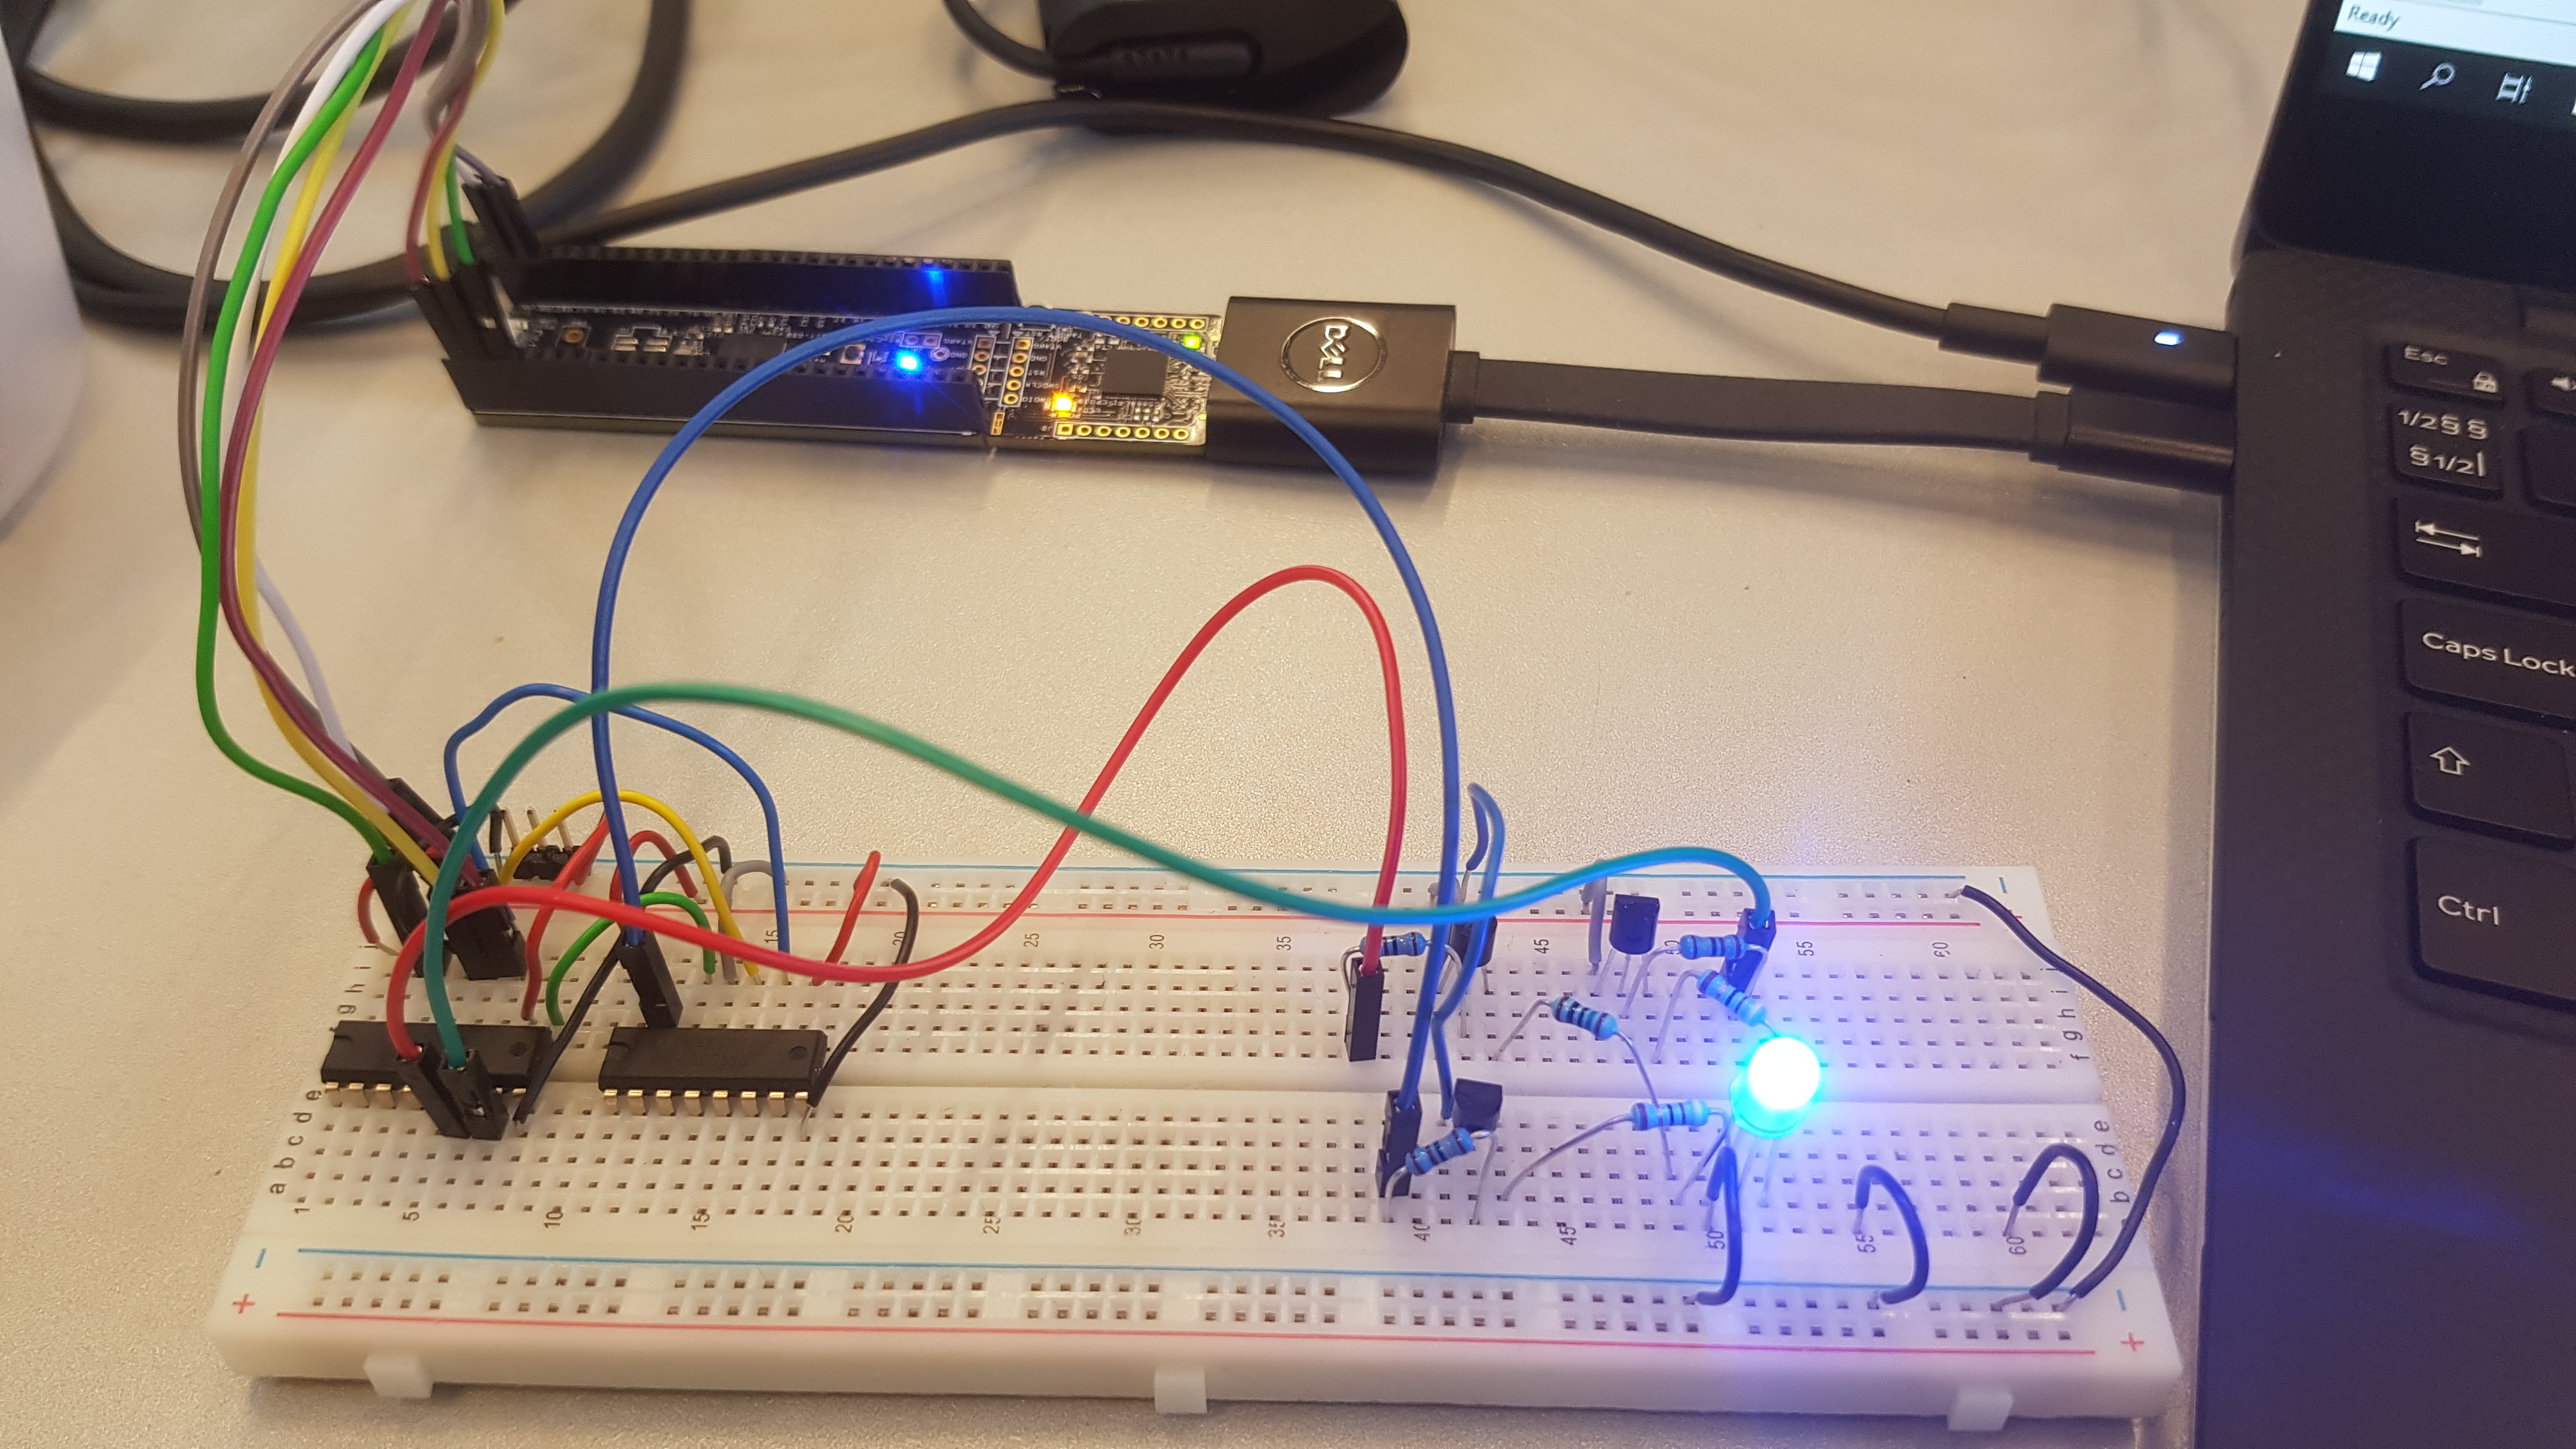
\includegraphics[width=\textwidth]{Modultest/CupLight/graphics/interface_test3.jpg}
    \caption{Test af controlLight(0,BLUE)}
    \label{fig:cuplight_blue_test3}
\end{figure}

Af figur \ref{fig:cuplight_red_test1},\ref{fig:cuplight_green_test2} og \ref{fig:cuplight_blue_test3} ses det, at det via interfacet er muligt at kontrollere forskellige RGB-leds til hver deres farve. Herudover laves der også tests, der viser forskellige farver, som LED'en kan lyse med. Her udvælges kun de klareste farver, som kan ses i de følgende figurer.

\begin{figure}[H]
    \centering
    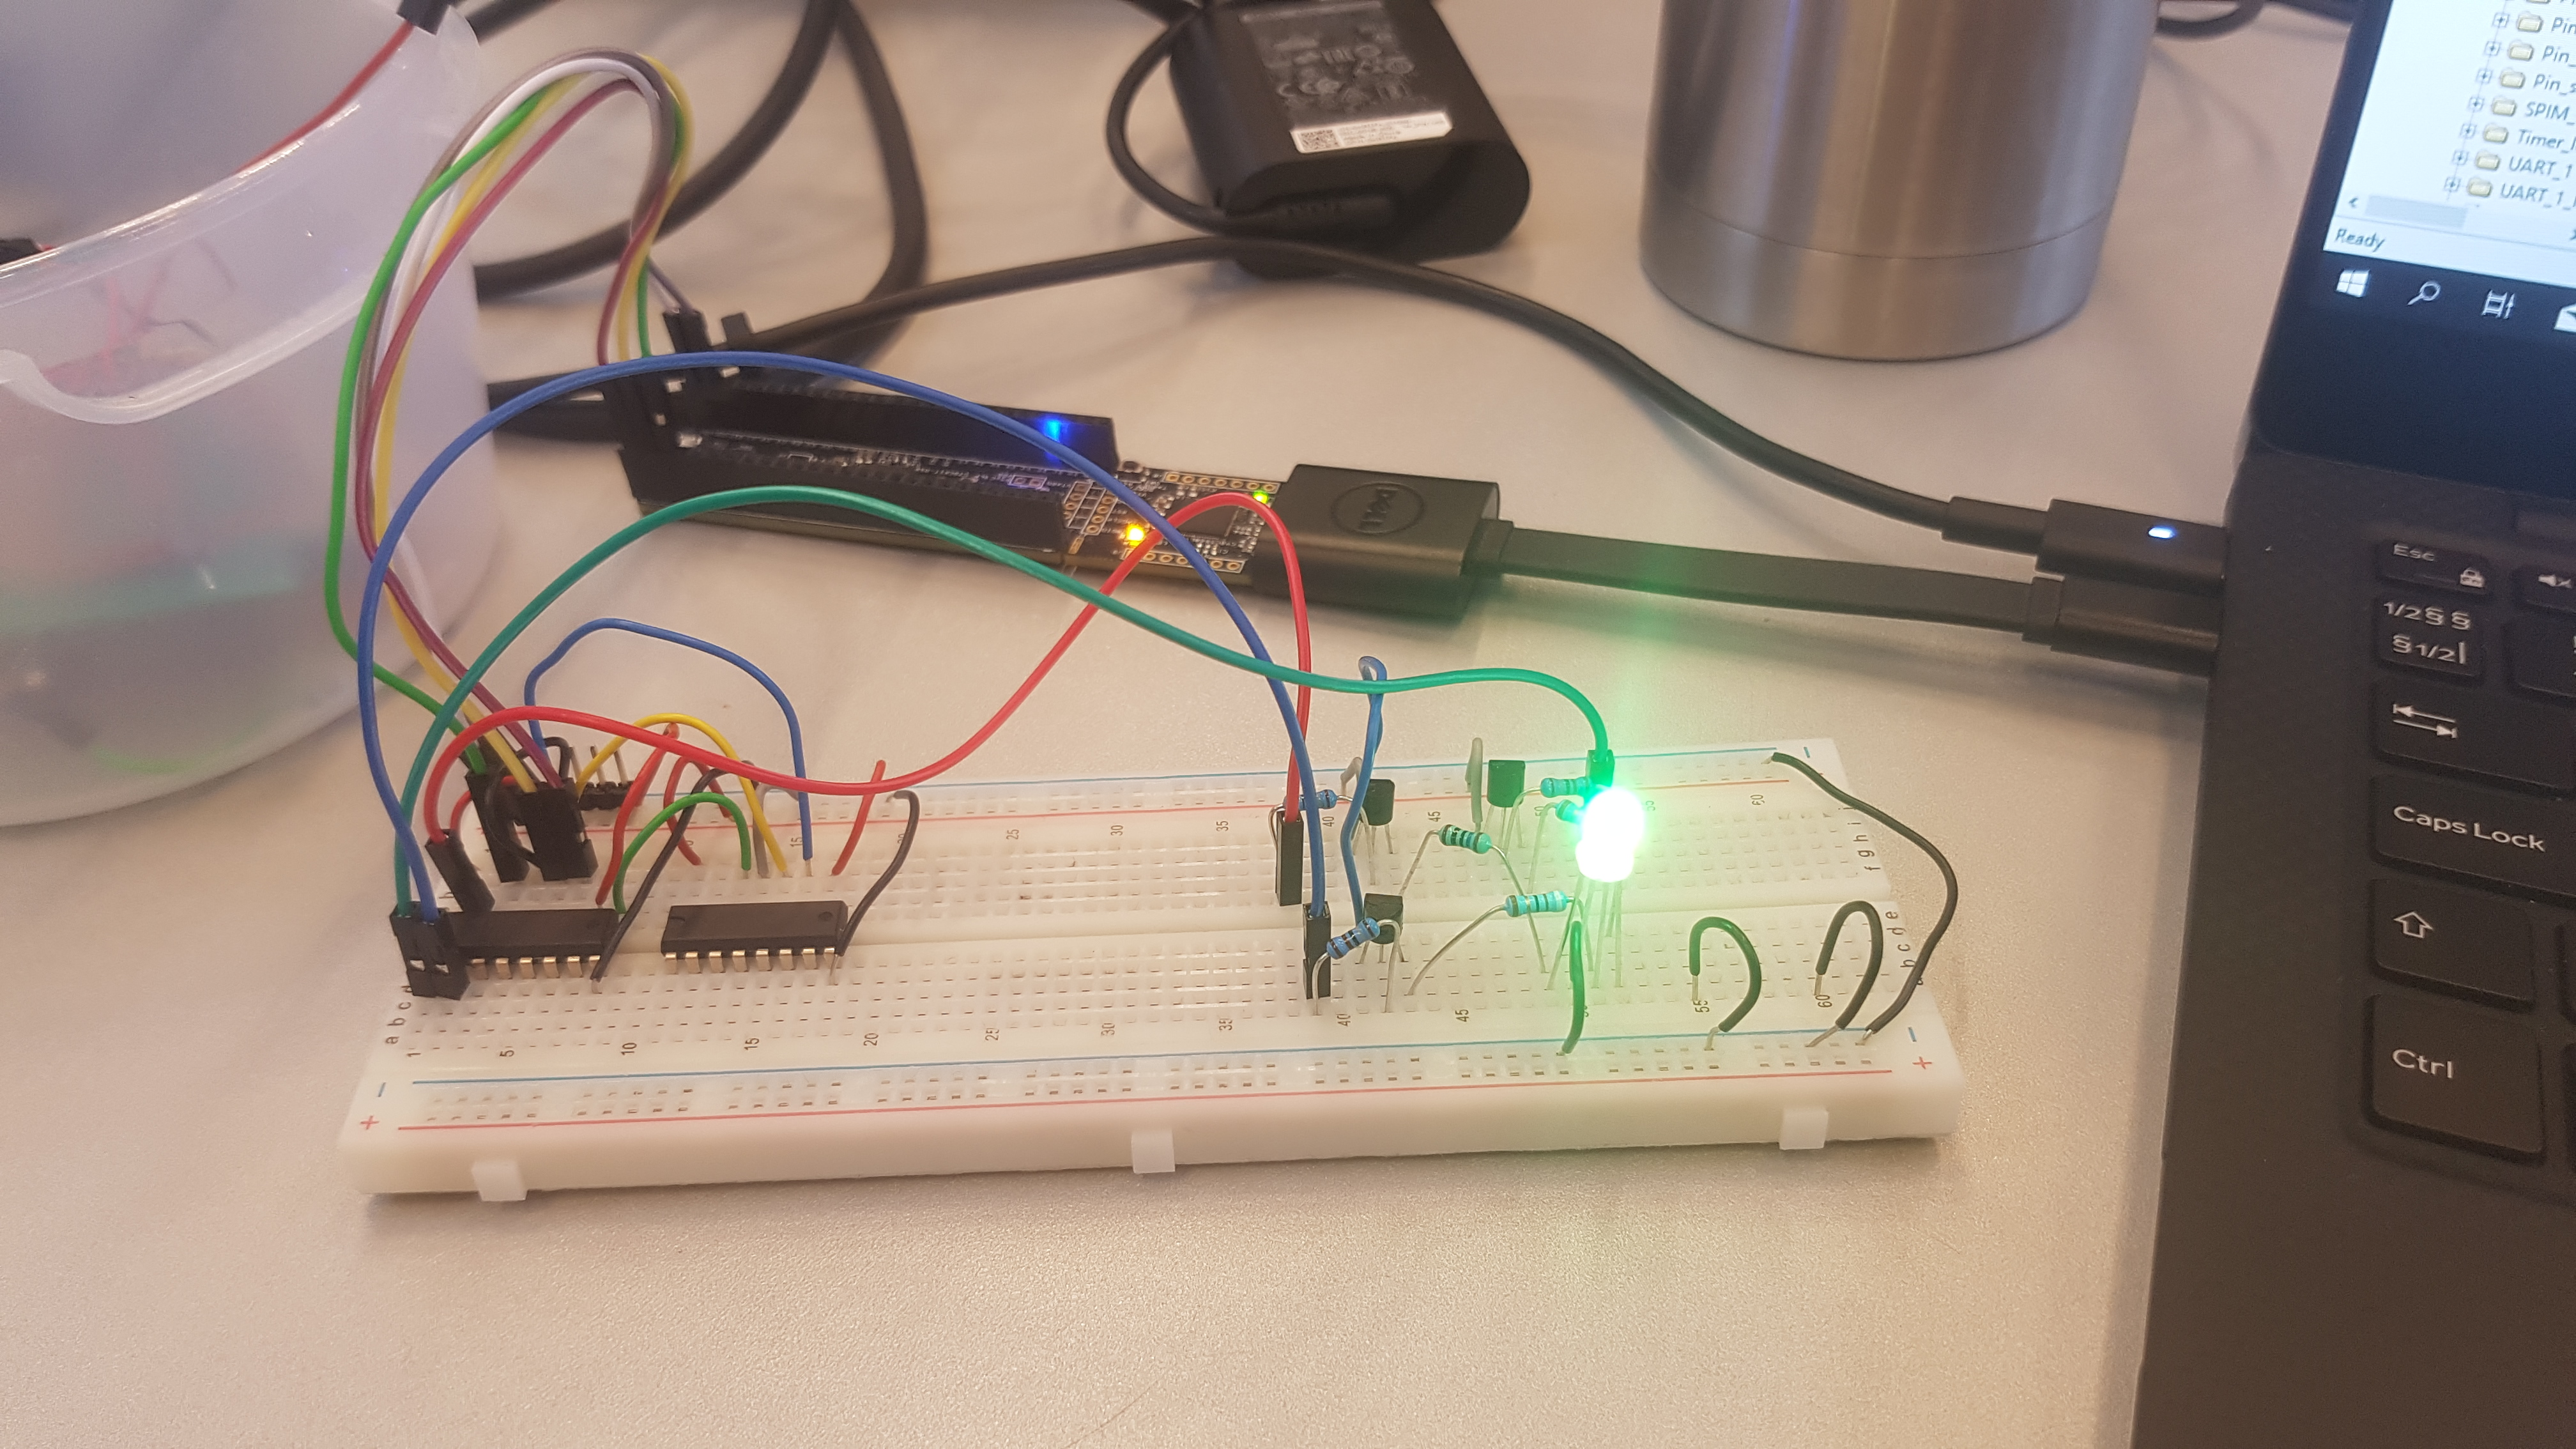
\includegraphics[width=\textwidth]{Modultest/CupLight/graphics/color_test1.jpg}
    \caption{Test af gul-farve}
    \label{fig:yellow_led}
\end{figure}

\begin{figure}[H]
    \centering
    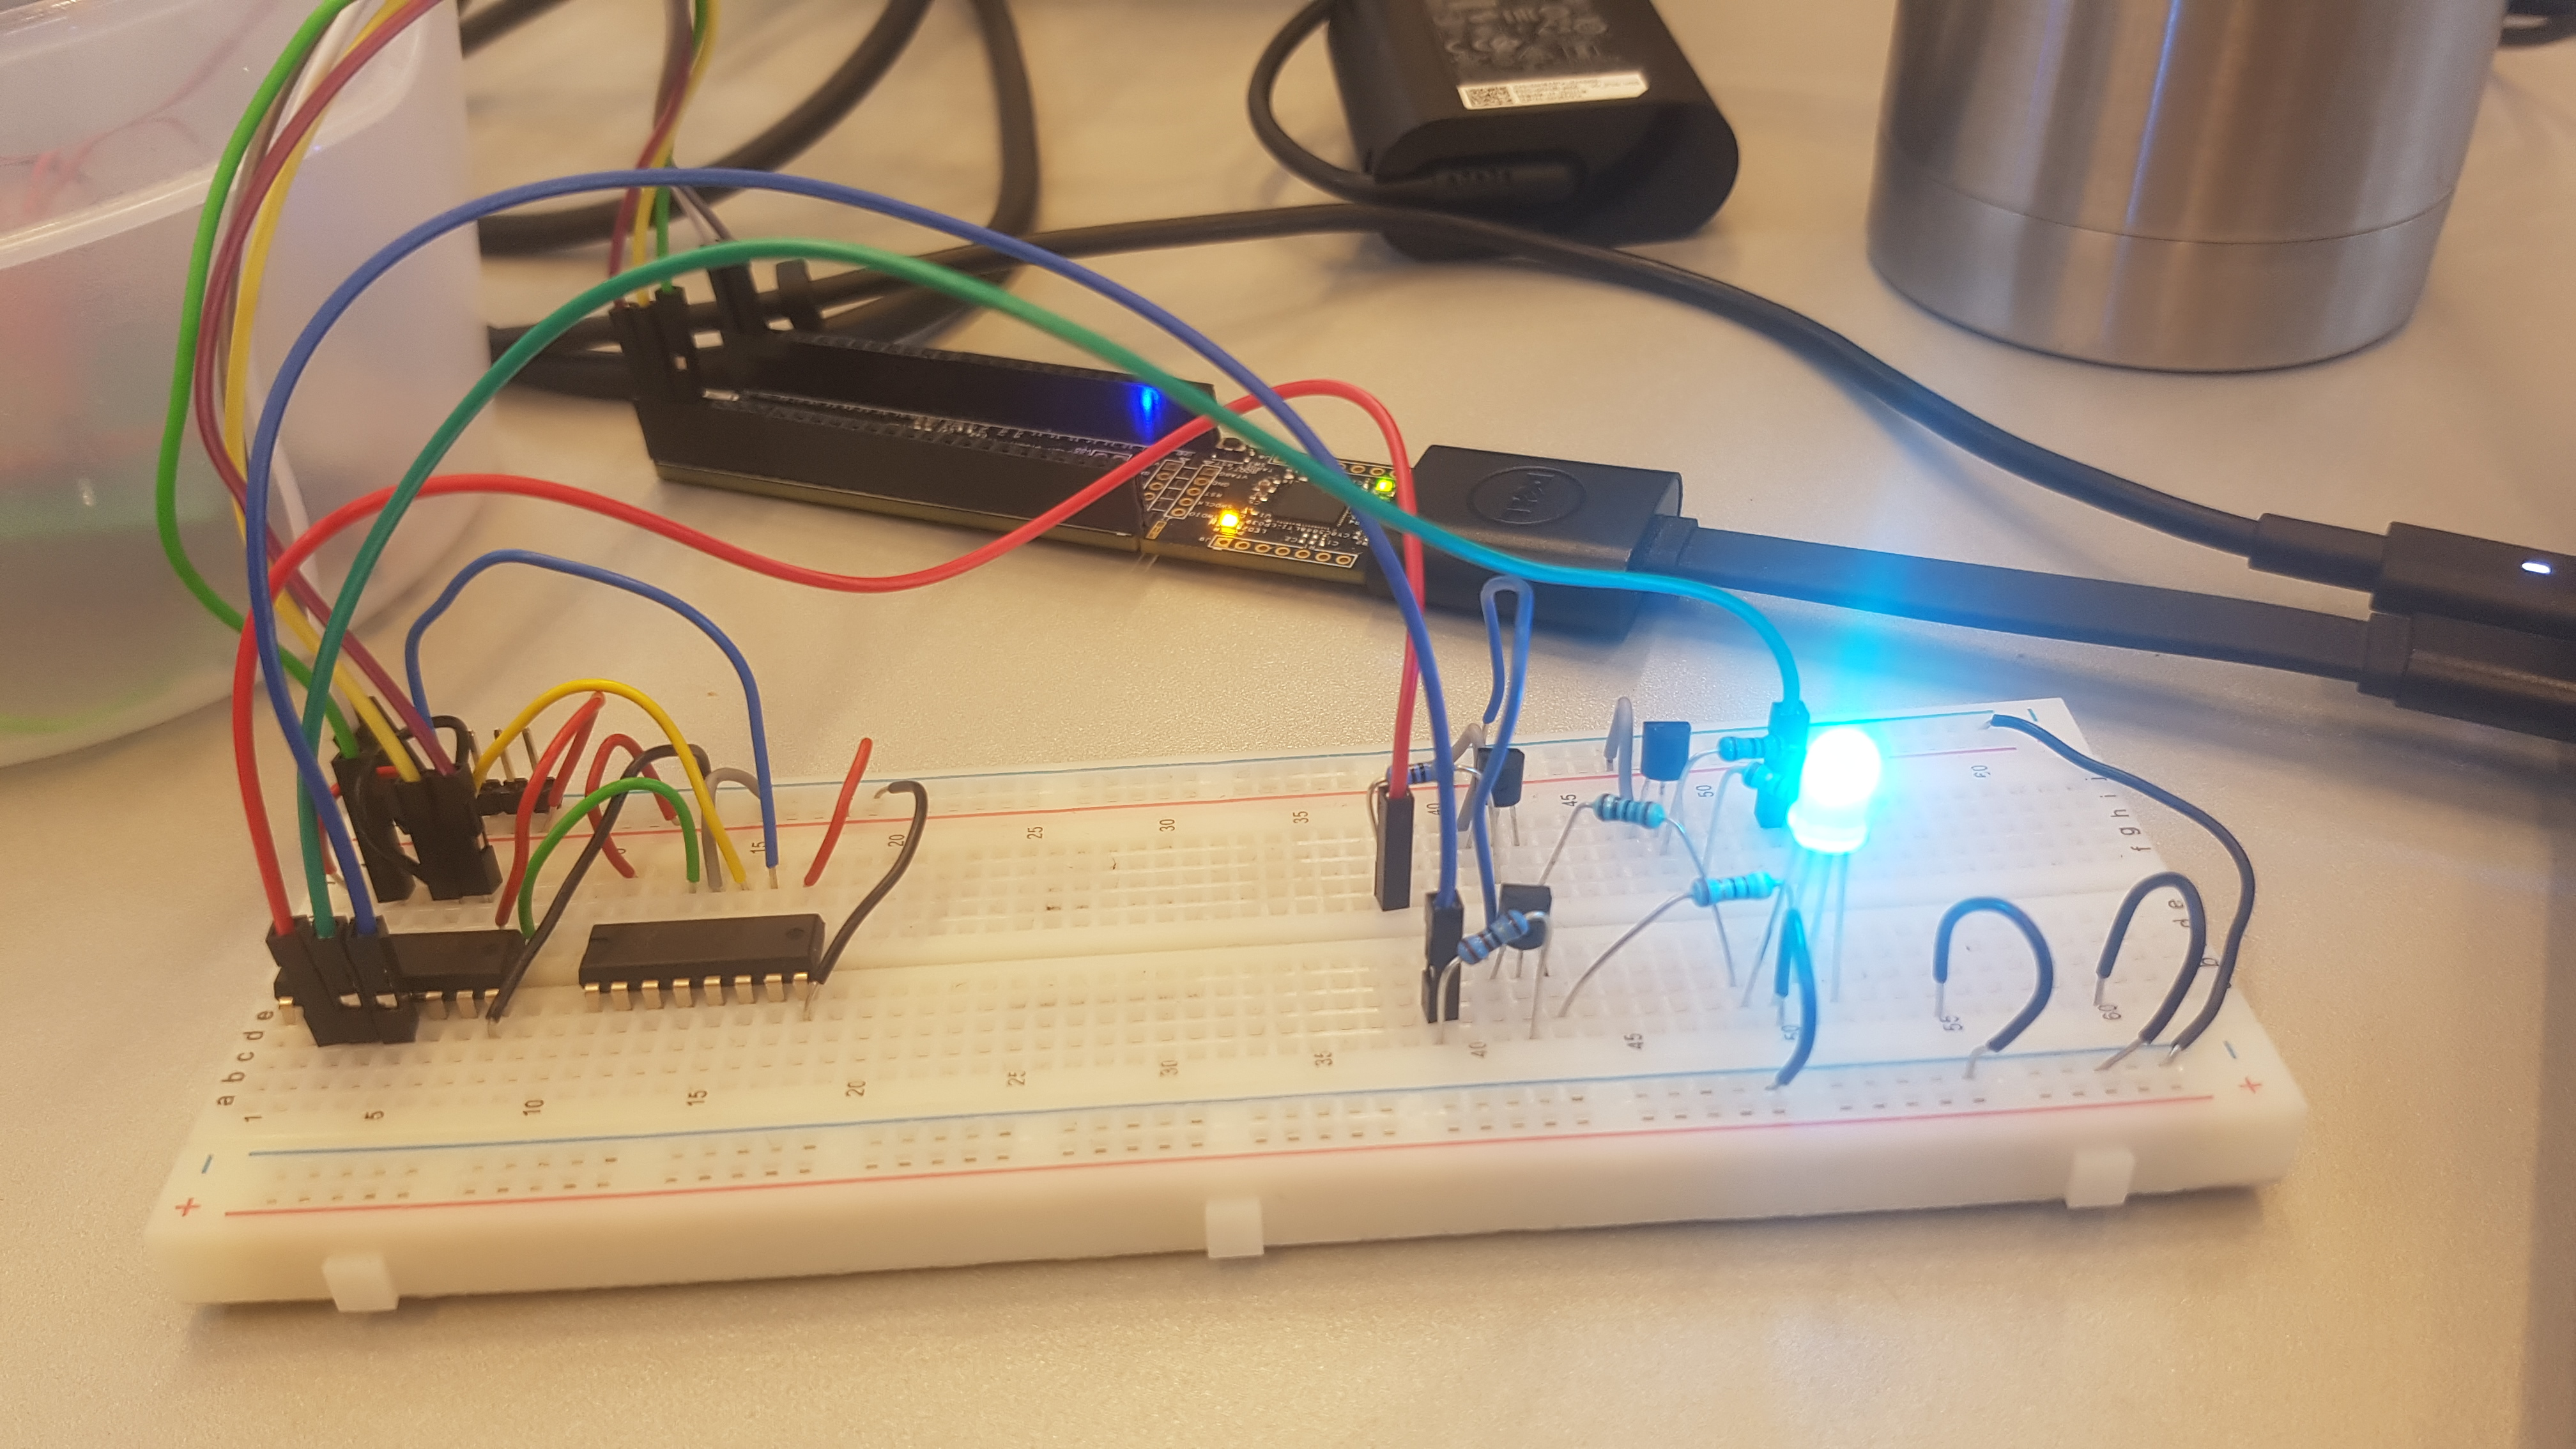
\includegraphics[width=\textwidth]{Modultest/CupLight/graphics/color_test2.jpg}
    \caption{Test af cyan-farve}
    \label{fig:cyan_led}
\end{figure}

\begin{figure}[H]
    \centering
    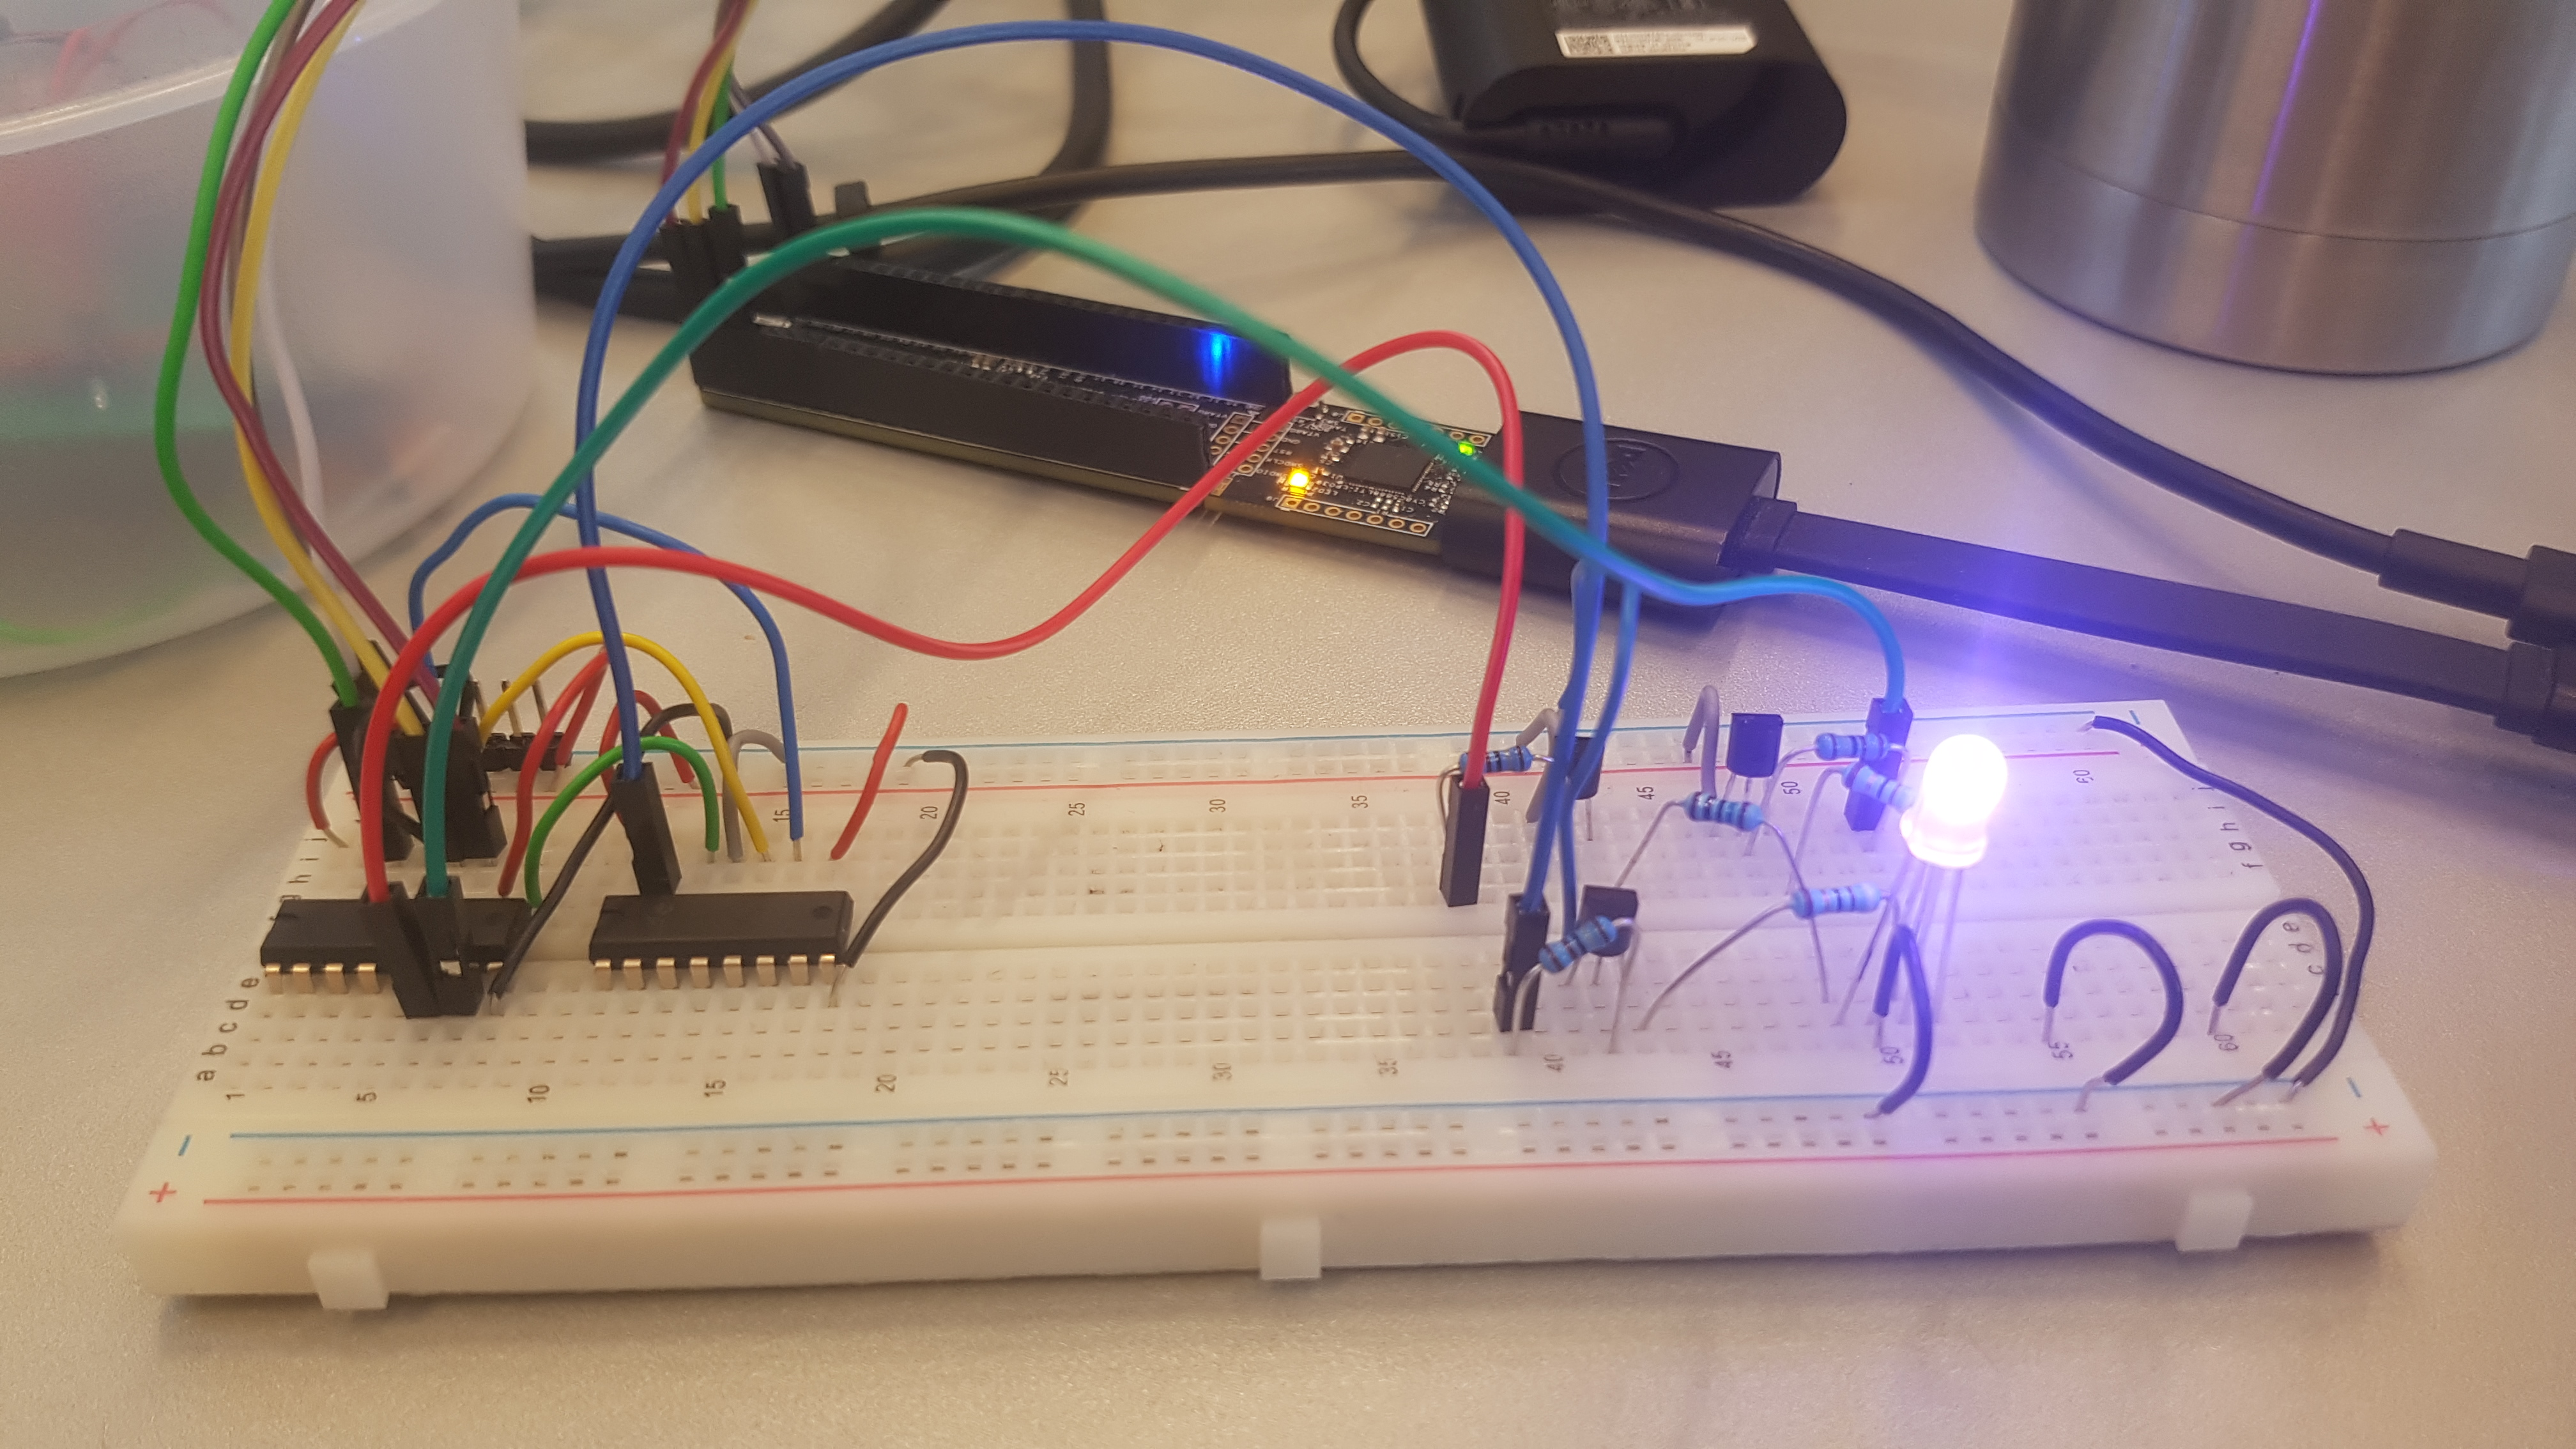
\includegraphics[width=\textwidth]{Modultest/CupLight/graphics/color_test3.jpg}
    \caption{Test af lilla-farve}
    \label{fig:purple_led}
\end{figure}

\begin{figure}[H]
    \centering
    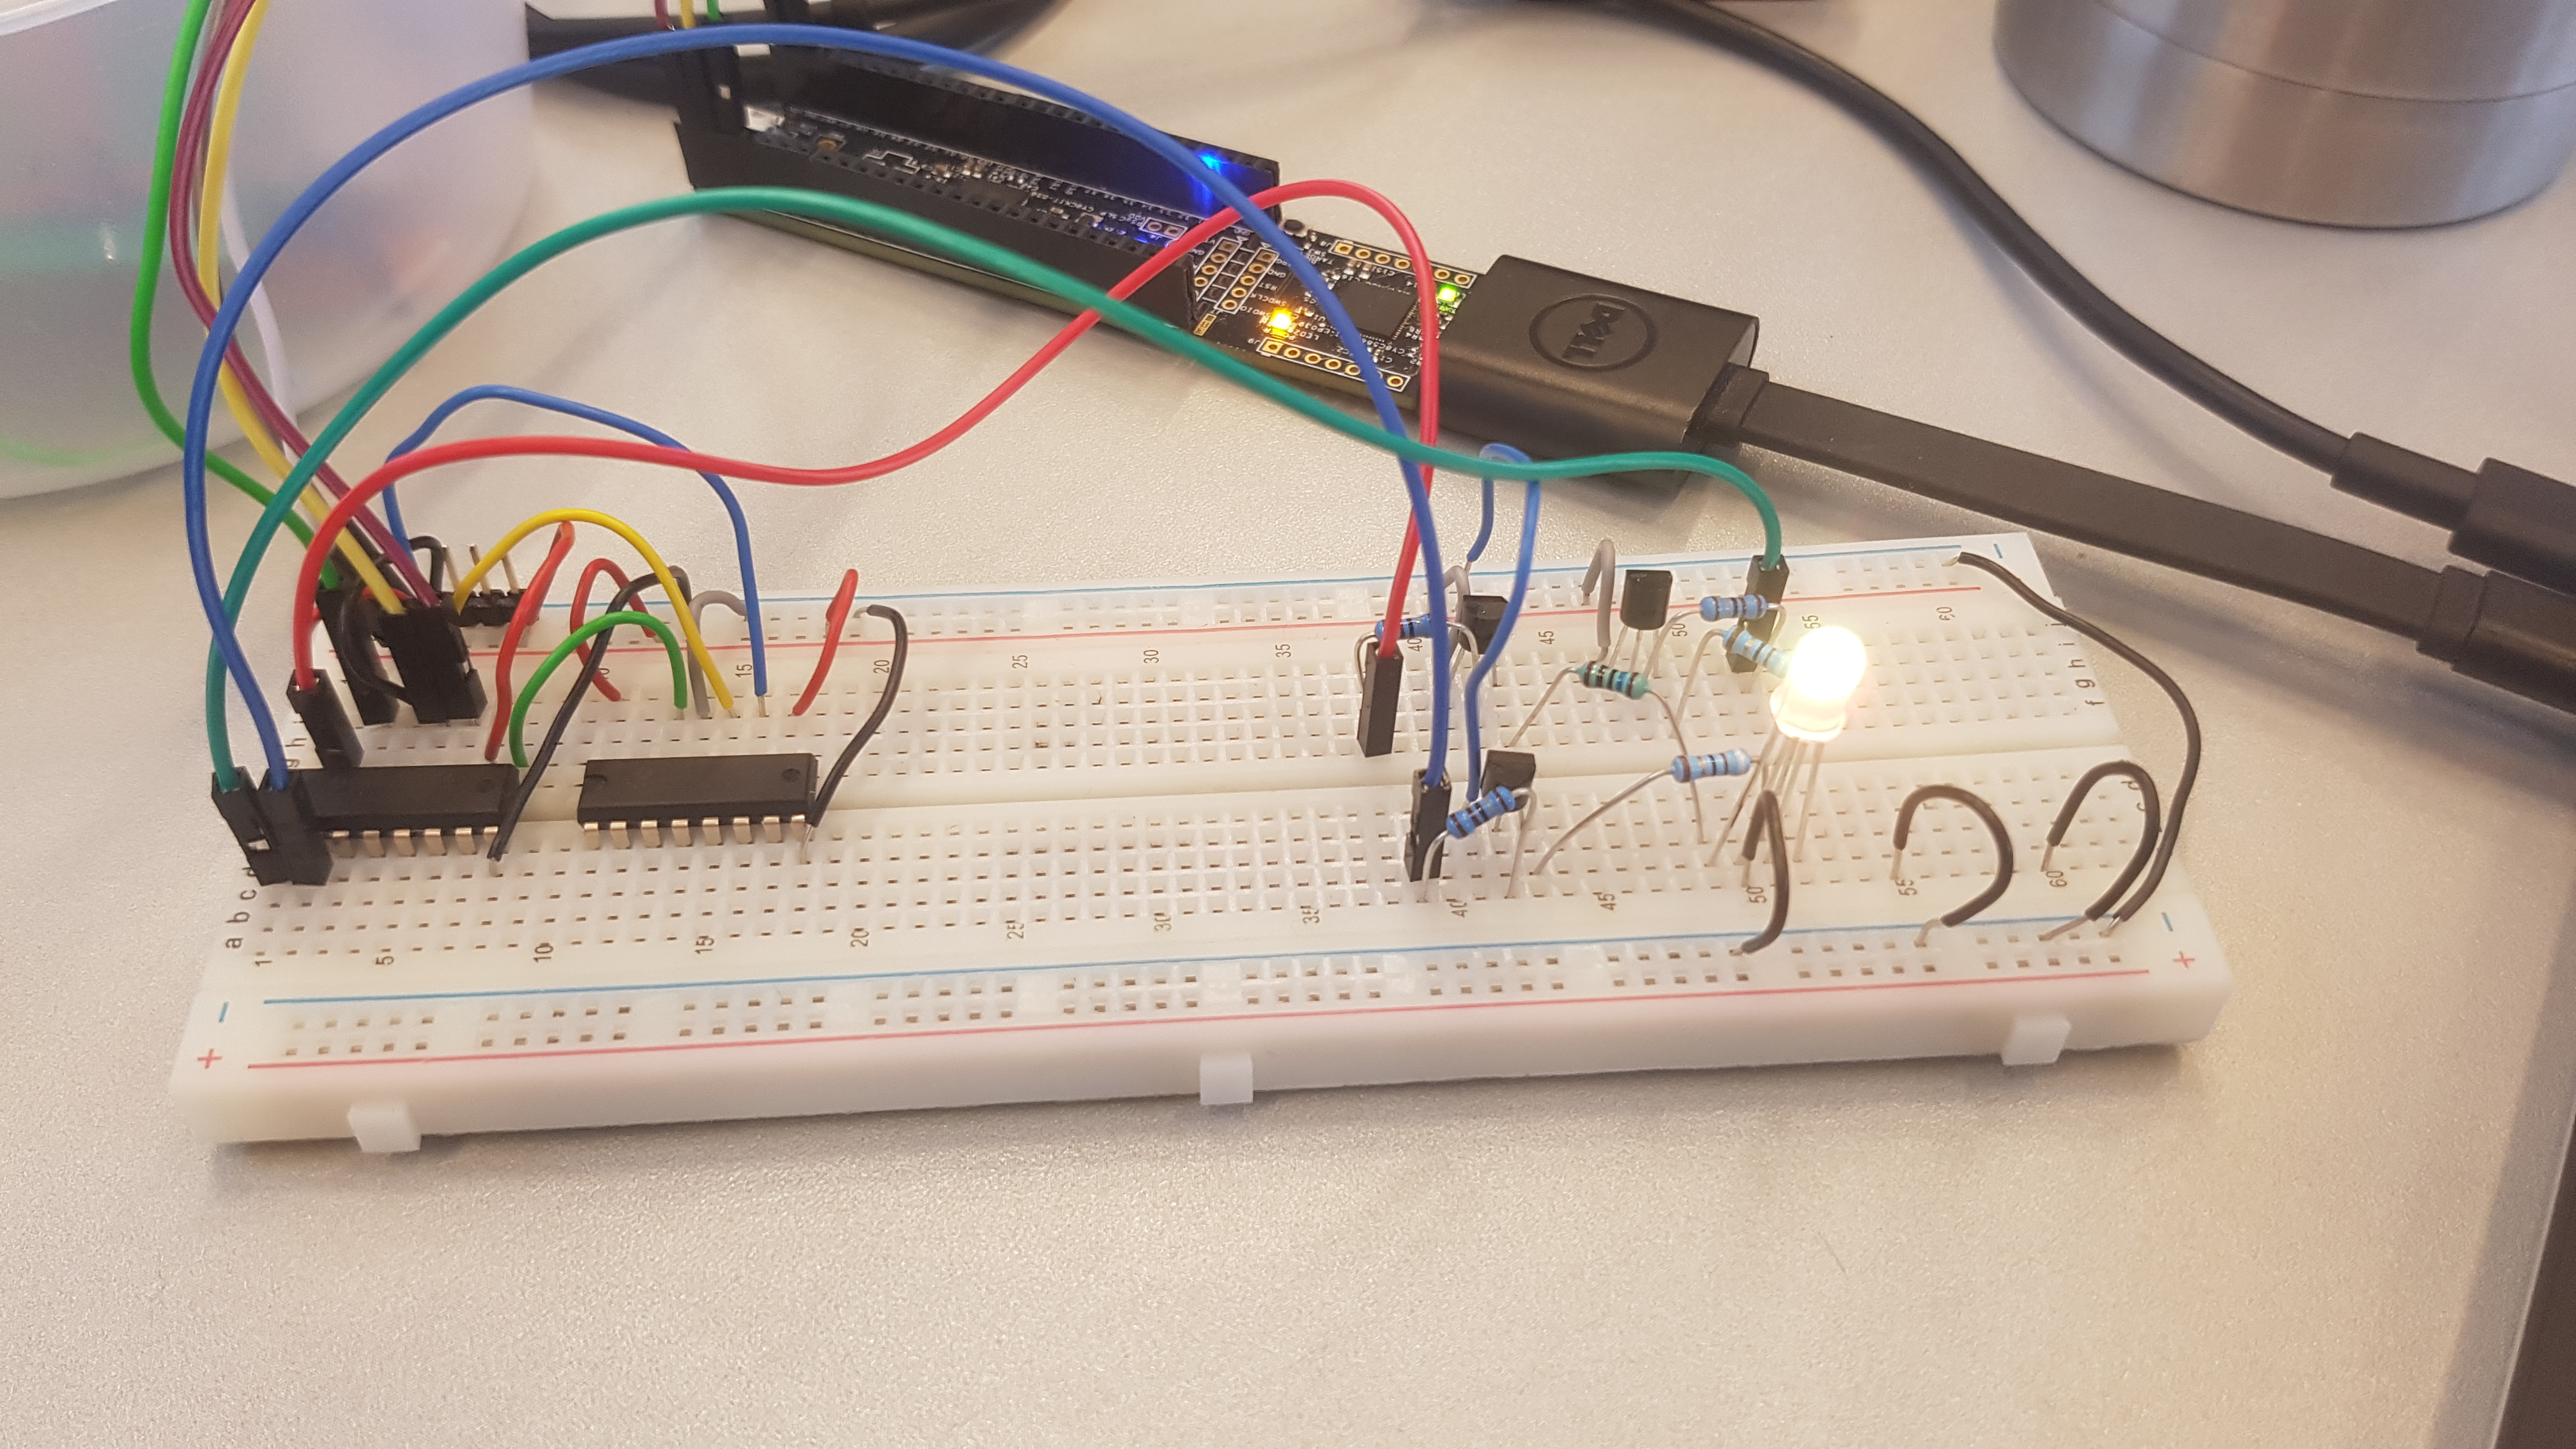
\includegraphics[width=\textwidth]{Modultest/CupLight/graphics/color_test4.jpg}
    \caption{Test af orange-farve}
    \label{fig:orange_led}
\end{figure}

\begin{figure}[H]
    \centering
    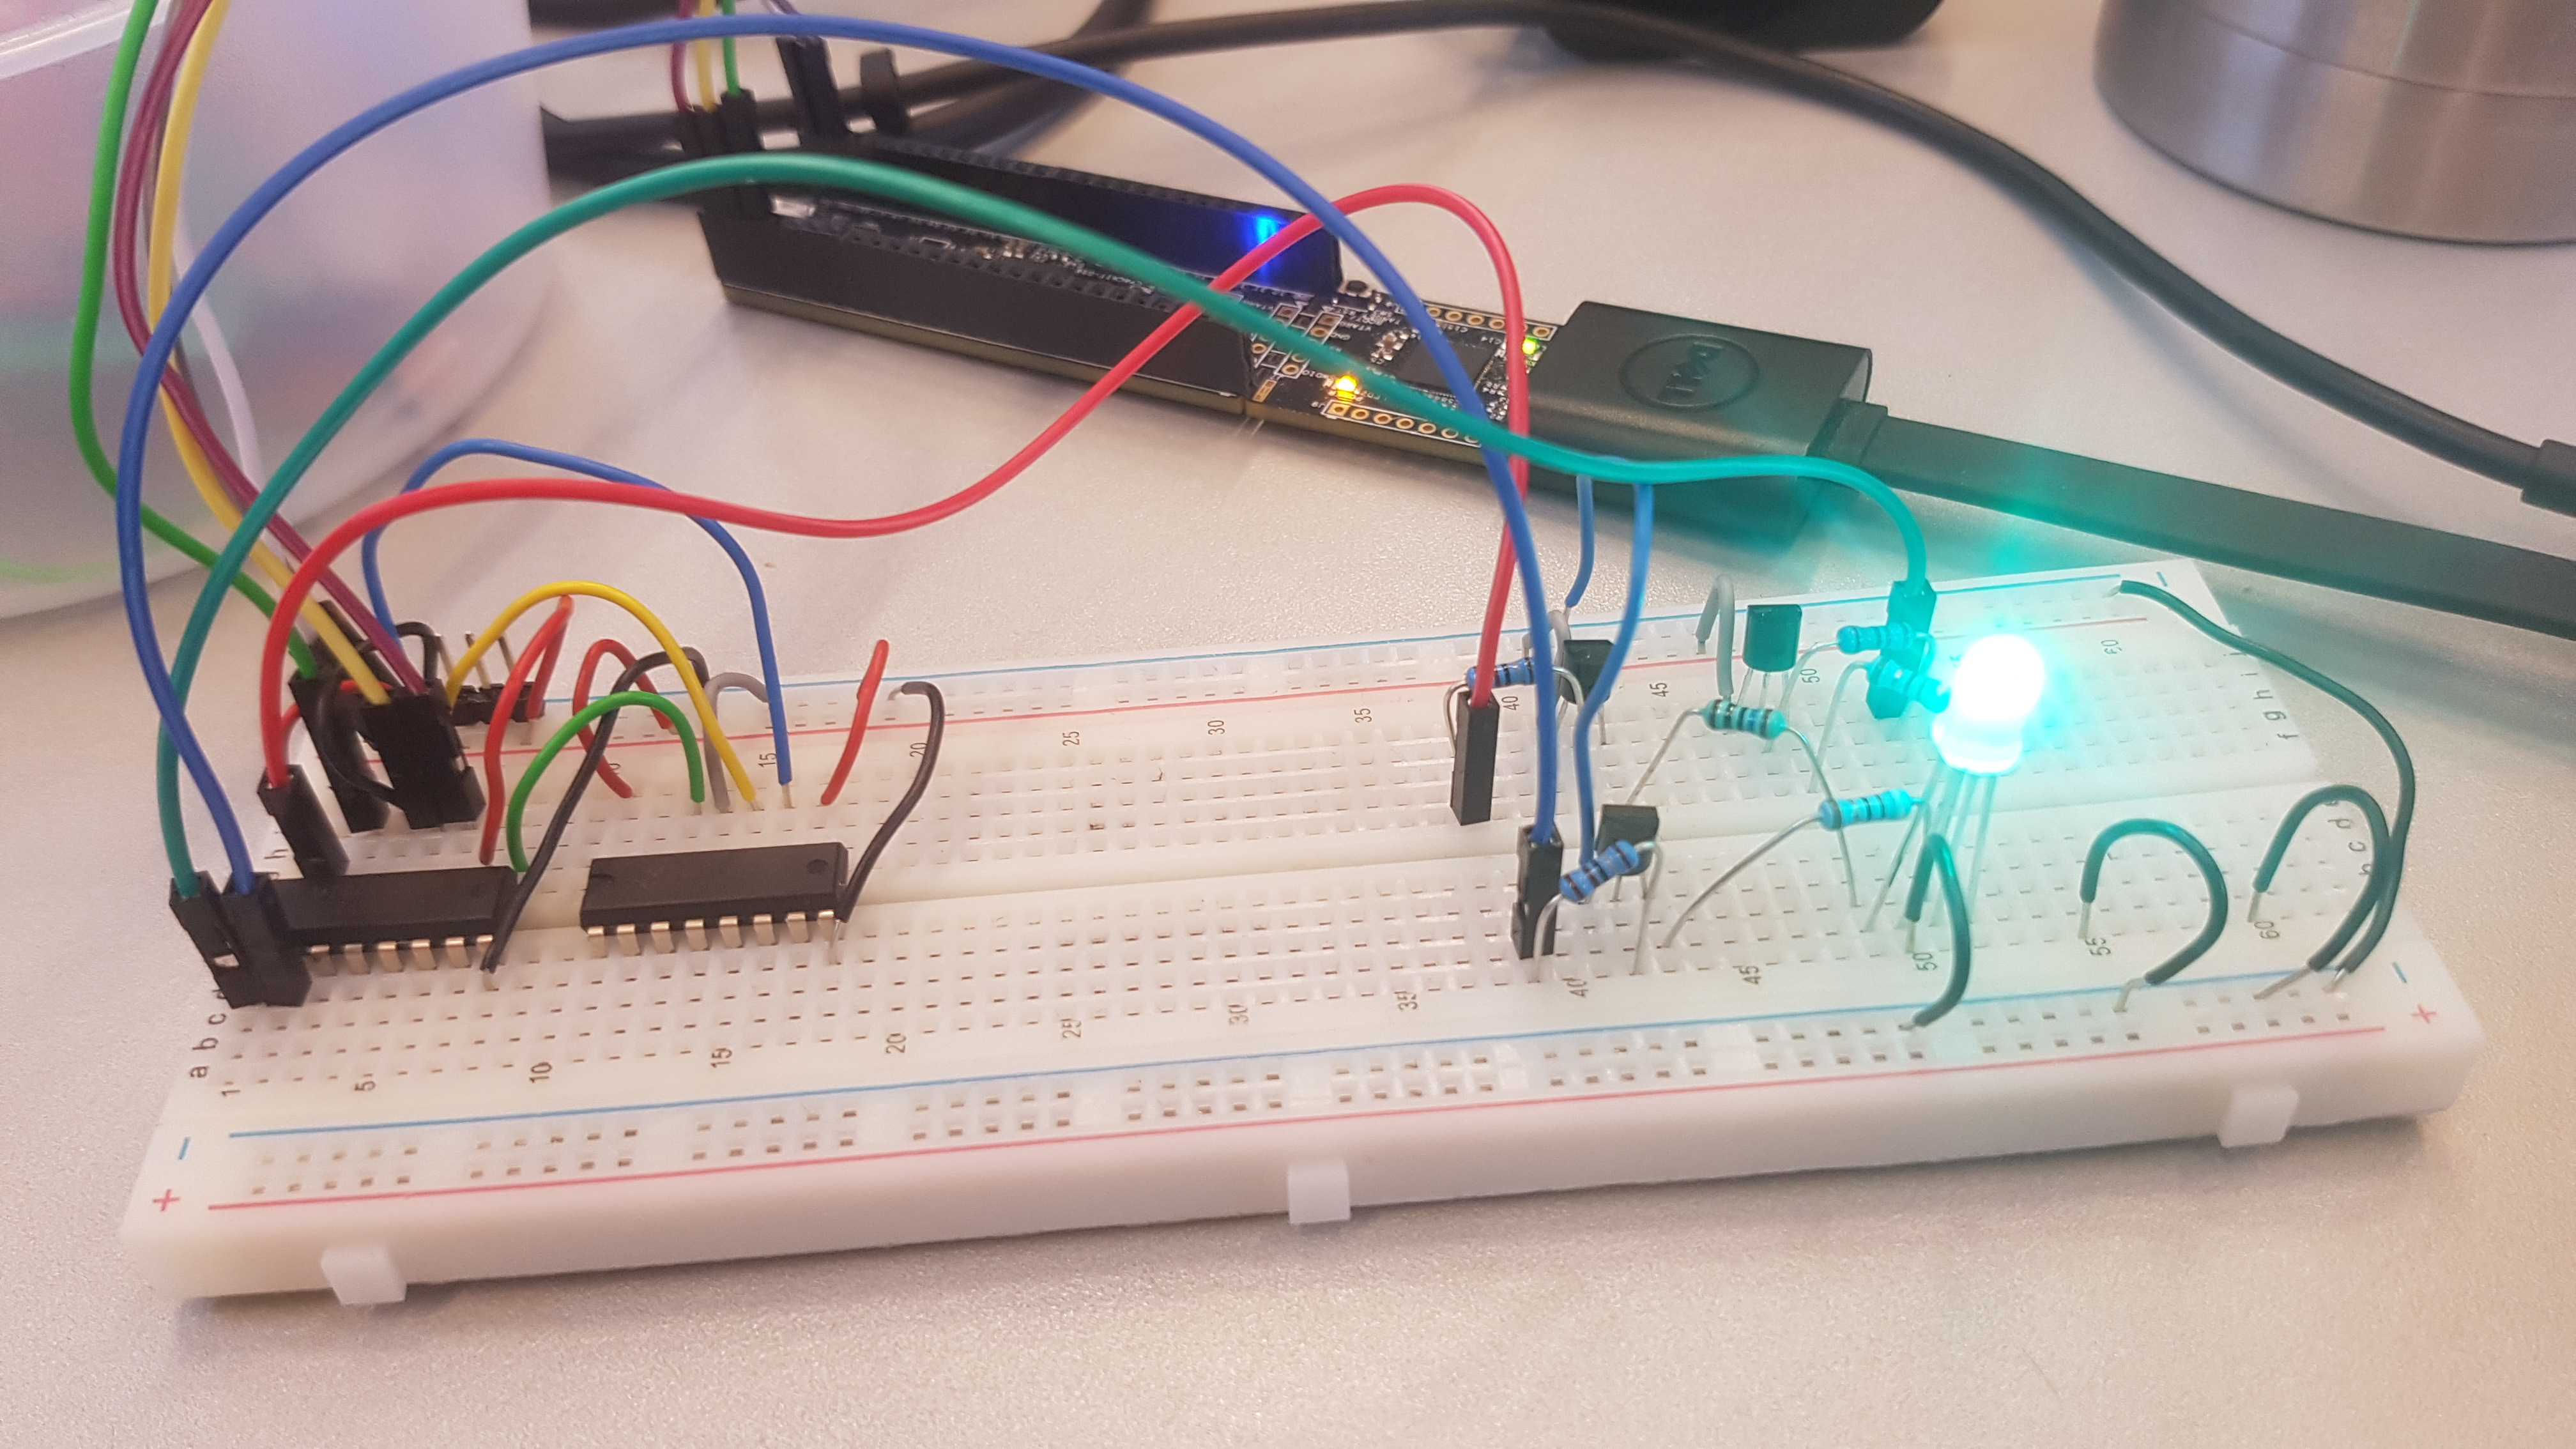
\includegraphics[width=\textwidth]{Modultest/CupLight/graphics/color_test5.jpg}
    \caption{Test af blågrøn-farve}
    \label{fig:bluegreen_led}
\end{figure}
Af figurene \ref{fig:yellow_led}, \ref{fig:cyan_led}, \ref{fig:purple_led}, \ref{fig:orange_led}, \ref{fig:bluegreen_led} kan det ses at de fleste farver rammer rimelig plet. Det kan også ses at det er den gule farve, der er dårligst i det, der er et grønligt skær. Det ses også at det altså er muligt at blande et bredt udvalg af farver. Flere farver blev testet på denne måde, bla. \textit{Hvid}, \textit{Gulgrøn} osv. Mange af farverne er selvfølgelig svære at definere, men det var muligt at se forskel, når der hoppes i steps af fem.\\\\

Modultesten for hele CupLight-modulet må siges at være lykkedes, da det både er muligt at styre mange PWM-signaler og derved også styre lys til mere end 10 forskellige farver. Skulle testene forbedres, så kunne der laves tests med flere lys forbundet til controller-kredsløbet. Derudover kunne der laves flere målinger for at bestemme konfidensniveauet af PWM-signalerne, men dette ville også kræve det var specificeret af kravene.


\end{document}